\documentclass [a4paper]{report}
\usepackage[english]{babel}
\usepackage[OT1]{fontenc}
\usepackage[utf8]{inputenc}
\usepackage{float}
\usepackage[center]{subfigure}
\usepackage{tabularx}
\usepackage{booktabs}
%\usepackage{algorithm}
%\usepackage{algorithmic}
%\usepackage{a4wide}
%\usepackage[pdftex,colorlinks=true,
%            pdfstartview=FitV,
%            linkcolor=blue,
%            citecolor=blue,
%            urlcolor=blue]{hyperref}
\usepackage[pdftex]{graphicx}
\usepackage{amsmath}
\usepackage{amssymb}
\usepackage{multirow}
%\usepackage{fancyhdr}
%\usepackage{multicol}
%\usepackage{times}
%\usepackage{index}
%\usepackage{wrapfig}

\newcommand{\mydef}{\stackrel{\text{def}}{\hbox{=}}} 

\begin{document}
\title{PhD Thesis}

\author{Stig Rune Jensen}
\date{\today}
\maketitle

\pagenumbering{roman}
\pagebreak
\ \\
\pagebreak
\tableofcontents
\chapter*{Acknowledgments}
I would like to express my gratitude to my supervisors, Luca Frediani, for teaching 
me what I know about quantum chemistry, and Tor Fl\aa, for teaching me the theory of
multiwavelets, and to them both for giving my a lot of freedom to persue my own 
interests and ideas. Luca has had a lot of things going on in his life during these 
years, but his door has always been open (literally, his home front door) if I ever 
needed advice or guidence.

I would like to give my sincere thanks to Jonas Jus\'{e}lius, who I had the privilege
to work with during my master's and the first years of my PhD. I might have known the
basic concepts of programming when I met you, but you turned me into a 
programmer. I miss our sharing of WTFs over a code that doesn't work, and I hope 
we get the chance to work together again soon. 

I would also like to mention the rest of the people at the HPC group who have been most 
accommodating in their support, by tweaking the hardware to suite my needs and by 
helping me cut in line when my jobs were to big for the queue.

I would like to give thanks to the CTCC group in Troms\o, to the people I have shared
office with, Jonas, Arnfinn and Krzysztof (and various random people at our guest spot).
To Peter and Antoine, who is/was also working on the multiwavelet project, and to Marco, 
Arnfinn, Roberto, Maarten, Luca (Oggioni) and Geir who joined me in various classes 
over the years (I have been the only student in several classes in the past, so your 
company has been appreciated), and to the rest of the lunch-eaters in the group. 
Finally, to the people at the CTCC in Oslo for many enjoyable joint meetings.

\pagebreak
\ 
\pagebreak

\pagenumbering{arabic}
\chapter{Introduction}
The work of this thesis has been contributing in the development of the 
program package MRChem, which is a code developed at the University of Tromsø 
\cite{Fossgaard} that is aiming at a fully numerical treatment of molecular 
systems, based on 
Density Functional Theory (DFT). There are currently a huge number of these
program packages available, each with more or less distinct features, and
what separates MRChem from all of these is the choice of basis functions.
While traditional computational chemistry programs use Gaussian type basis sets
for their efficient evaluation of two- and four-electron integrals, MRChem is
based on the multiresolution wavelet basis.\\

\noindent
Wavelet theory is a rather young field of mathematics, first appearing in the
late 1980s. The initial application was in signal theory \cite{Strang} but in
the early 90s, wavelet-based methods started to appear for the solution of
PDEs and integral equations \cite{Beylkin90}\cite{Alpert93}, and in recent 
years for application in electronic structure calculations
\cite{Harrison}\cite{Niklasson}\cite{Arias}.

\subsection*{The Kohn-Sham equations}
In the Kohn-Sham \cite{Kohn-Sham} formulation of DFT the eigenvalue equations 
for the electronic structure can be written
\begin{equation}
	\label{eq:Kohn-Sham}
	\lbrack
	-\frac{1}{2}\nabla^2+V_{eff}(\boldsymbol{r})\rbrack\psi_i(\boldsymbol{r}) =
	\epsilon_i\psi_i(\boldsymbol{r})
\end{equation}
where the effective potential is the collection of three terms
\begin{equation}
	\label{eq:Veff}
	V_{eff}(\boldsymbol{r}) =
	V_{ext}(\boldsymbol{r})+V_{coul}(\boldsymbol{r})+V_{xc}
\end{equation}
where the external potential $V_{ext}$ is usually just the electron-nuclear
attraction, the Coulomb potential $V_{coul}$ is the electron-electron
repulsion and $V_{xc}$ is the exchange-correlation potential which (in
principle) includes all non-classical effects. The functional form of $V_{xc}$
is not known.\\

\noindent
The nuclear charge distribution is a collection of point charges, and the 
nuclear potential has the analytical form
\begin{equation}
	V_{nuc}(\boldsymbol{r}) = -\sum_{\alpha=1}^{N_{nuc}}
	\frac{Z_{\alpha}}{|\boldsymbol{r}-\boldsymbol{r}_{\alpha}|}
\end{equation}
The electronic charge distribution is given by the Kohn-Sham orbitals
\begin{equation}
	\rho(\boldsymbol{r}) = 2\sum_{i=1}^{N_e/2} |\psi_i(\boldsymbol{r})|^2
\end{equation}
assuming a closed shell system with double occupancy. The electronic potential 
is now given as the solution of the Poisson equation
\begin{equation}
	\nabla^2 V_{coul}(\boldsymbol{r}) = 4\pi\rho(\boldsymbol{r})
\end{equation}
where the orbital-dependence of the potential makes eq.(\ref{eq:Kohn-Sham}) a set
of non-linear equations that is usually solved self-consistently. 
The current work will not be concerned with the solution of the Kohn-Sham
equations, but is rather a precursor to this where some building blocks
required for the DFT calculations are prepared, in particular the solution of 
the Poisson equation.

\subsection*{The Poisson equation}
Solving the Poisson equation for an arbitrary charge distribution is a 
non-trivial task, and is of major importance in many fields of science, 
especially in the field of computational chemistry. A huge effort has been put 
into making efficient Poisson solvers, and usual real-space approaches includes
finite difference (FD) and finite element (FE) methods. FD is a a grid-based
method, which is solving the equations iteratively on a discrete grid of 
pointvalues, while FE is expanding the solution in a basis set, usually by
dividing space into cubic cells and allocate a polynomial basis to each cell.\\

\noindent
It is a well-known fact that the electronic density in molecular systems
is rapidly varying in the vicinity of the atomic nuclei, and a usual problem
with real-space methods is that an accurate treatment of the system requires
high resolution of gridpoints (FD) or cells (FE) in the nuclear regions.
Keeping this high resolution uniformly througout space would yield unnecessary
high accuracy in the interatomic regions, and the solution of the Poisson
equation for molecular systems is demanding a \emph{multiresolution} framework 
in order to achieve numerical efficiency.\\

\noindent
There are ways of resolving these issues using multigrid techniques, and a nice
overview of these methods is given by Beck \cite{Beck}, but this thesis is 
concerned with a third way of doing real-space calculations, one where the
multiresolution character is inherent in the theory, namely using wavelet
bases.\\

\noindent
At this point MRChem is basically a Poisson solver. It has the capabilities of 
representing arbitrary functions in the multiwavelet basis, and calculate the 
potential originating from these functions. This is the result of the work by
\cite{Fossgaard}. The current work includes the
implementation of some basic arithmetic operations involving these function
representations, where the space adaptivity of the grid and strict error
control will be important topics. We will also look at some possible 
optimizations of the existing code, where computational efficiency, memory
requirements and linear scaling with respect to system size will be important.
\\

\noindent
The thesis is split in two parts; theory and implementation. The theory part
gives a brief overview of the mathematical theory of multiwavelets, from the
basic concept of multiresolution analysis, to the representation of functions 
and operators in the multiwavelet basis, and ultimately to the solution of the
Poisson equation. The implementation part gives a short description of the
data structures and algorithms used in the MRChem program, and some details of
how the mathematical theory is implemented in practice. Some numerical results
are given to show the capabilities and performances of the code.


\subsection{Multiwavelets}
In the construction of the multiwavelet basis we start with a simple set of 
orthogonal polynomials $\lbrace\phi_j\rbrace_{j=0}^k$ of order $k$ on the unit 
interval. This can be e.g. the Legendre polynomials shifted to the unit interval. 
If this basis turns out to be too crude to accurately describe the function, we 
split the interval and double the number of basis functions by dilating and 
translating the original basis to both subintervals
\begin{equation}
    \phi_{j,l}^1(x) = 2^{1/2}\phi_j(2x - l), \qquad l = 0,1
\end{equation}
The polynomials are defined only on their respective intervals, so basis functions 
at different translations are by construction orthogonal. The splitting procedure 
can be continued until we have reached a scale $n$ where we are satisfied with the 
accuracy of the representation. At this level of refinement the unit interval has 
been split in $2^n$ intervals, each of size $2^{-n}$ containing a dilated and 
translated version of the original $k$-order basis
\begin{equation}
    \label{eq:two_scale}
    \phi_{j,l}^n(x) = 2^{n/2}\phi_j(2^nx - l), \qquad l = 0,\dots,2^n-1
\end{equation}
These are the so-called scaling functions, and they span the scaling space 
$\scalingspace{n}$. This basis can be used to represent any square integrable 
function to any finite accuracy by adjusting the polynomial order $k$ and/or the 
level of refinement $n$. With this construction, it is easy to verify that each 
scaling space is fully contained in all scaling spaces of higher resolution, and 
we have the following relation
\begin{equation}
    \label{eq:MRA}
    \scalingspace{0} \subset \scalingspace{1} \subset \ldots
    \subset \scalingspace{n} \subset \ldots
\end{equation}
In addition to scaling functions, the multiwavelet basis consists of another set 
of piecewise polynomials, the wavelet functions $\psi_{j,l}^n$, that span the 
wavelet space $\waveletspace{n}$. This space is defined as the orthogonal 
complement of $\scalingspace{n}$ in $\scalingspace{n+1}$
\begin{equation}
    \label{eq:wavelet-def}
    \waveletspace{n} \oplus \scalingspace{n} = \scalingspace{n+1}
\end{equation}
The wavelet functions satisfy the same two-scale relation as the scaling functions 
in Eq.~(\ref{eq:two_scale}).
\\
\\
\noindent
The extension to three dimensions is done using a standard tensor-product structure, 
where we get a basis of $(k+1)^3$ pure scaling functions on each cubic cell 
\begin{equation}
    \label{eq:tensor_basis}
    \Phi^n_{ijk}(x,y,z) = \phi^n_i(x)\phi^n_j(y)\phi^n_k(z)
\end{equation}
and we note that from the definition of the wavelet space in Eq.~(\ref{eq:wavelet-def}) 
we get a total of $(2^3-1)(k+1)^3$ wavelet functions on each cell (all combinations in 
Eq.~(\ref{eq:tensor_basis}) that contain at least one wavelet function), and it becomes 
apparent that the treatment of more than three dimensions is problematic as the size of 
the basis grows exponentially in the dimension.


\pagebreak

\chapter{Multiresolution analysis}\label{chap:mathematics}
In this chapter a general introduction to multiwavelet theory will be given through 
the concept of multiresolution analysis (MRA)\footnote{Mallat uses the term 
multiresolution \emph{approximation}, but in this work we will use multiresolution 
\emph{analysis}, as it is more commonly used in the literature.}, that was developed 
by Mallat\cite{Mallat:1989} and Daubechies\cite{Daubechies:1988} in the late 1980s. 
A detailed description of MRAs can be found in Keinert\cite{Keinert:2004}, from 
which a brief summary of the key issues are given in the following, with the 
difference that we limit our discussion to the unit interval instead of the real line.

\section{Orthogonal MRA}
A multiresolution analysis of $L^2([0,1])$ is an infinite nested sequence of subspaces
\begin{equation}
    \label{eq:MRA}
    \scalingspace{0}\subset \scalingspace{1}\subset \cdots \subset 
	\scalingspace{n}\subset \cdots \subset L^2([0,1])
\end{equation}
with the following properties
\begin{enumerate}
    \item $\bigcup_{n=0}^{\infty}\scalingspace{n}\ is\ dense\ in\ L^2([0,1])$.
    \item $f(x) \in \scalingspace{n} \Longleftrightarrow f(2x) \in \scalingspace{n+1}
    	\ ,\ \forall n \in \mathbb{N}$.
    \item $f(x) \in \scalingspace{n} \Longleftrightarrow f(x-2^{-n}l) \in 
	\scalingspace{n}\ ,\ \forall n \in \mathbb{N},\ 0 \leq l \leq 2^n - 1.$
    \item There exists a function vector $\scalingvec$ in $L^2([0,1])$ of length
	$k+1$ such that the vector components $\scaling_i$ forms a basis of 
	\scalingspace{0}. 
\end{enumerate}
This means that if we can construct a basis of \scalingspace{0}, which consists of 
only $k+1$ functions, we can construct a basis of \emph{any} space \scalingspace{n}, 
by simple compression (by a factor of $2^n$, property 2), and translations (to all 
dyadic grid points at scale $n$, property 3), of the original $k+1$ functions, and 
by increasing the scale $n$, we are approaching a complete basis of $L^2([0,1])$. 
Since $\scalingspace{n} \subset \scalingspace{n+1}$ the basis functions of 
\scalingspace{n} can be expanded in the basis of \scalingspace{n+1}
\begin{equation}
    \label{eq:twoscalescaling}
    \scaling^n_{i,l}(x) \mydef 2^{n/2}\scaling_i(2^nx-l) = 
	\sum_{m=0}^{2^n-1} \sum_{j=0}^k H_{ij}^{(m)} \scaling^{n+1}_{j,m}(x)
\end{equation}
where the $H^{(m)}$s are the so-called filter matrices that describes the 
transformation between different spaces \scalingspace{n}. The MRA is called 
orthogonal if 
\begin{equation}
    \label{eq:orthogonality}
    \langle \scaling_{i,l}^n, \scaling_{j,m}^n \rangle = \delta_{i,j}\delta_{l,m}
\end{equation}
This orthogonality condition means that the 
functions are orthogonal both within one function vector and through all 
possible translations on one scale, but \emph{not} through the different scales.

Complementary to the nested sequence of subspaces \scalingspace{n}, we can define 
another series of spaces \waveletspace{n} that complements \scalingspace{n} in 
\scalingspace{n+1}
\begin{equation}
    \label{eq:MRAcomplement}
    \scalingspace{n+1} = \scalingspace{n} \oplus \waveletspace{n}
\end{equation}
where there exists another function vector $\waveletvec$ of lenght $k+1$ that, with 
all its translations on scale $n$ form a basis for \waveletspace{n}.
Analogously to Eq.~(\ref{eq:twoscalescaling}) the function vector can be expanded 
in the basis of \scalingspace{n+1}
\begin{equation}
    \label{eq:twoscalewavelet}
    \wavelet^n_{i,l}(x) \mydef 2^{n/2}\wavelet_i(2^nx-l) = 
	\sum_{m=0}^{2^n-1} \sum_{j=0}^k G_{ij}^{(m)}\scaling_{j,m}^{n+1}(x)
\end{equation}
with filter matrices $G^{(m)}$. In orthogonal MRA the functions $\waveletvec$ fulfill 
the same othogonality condition as Eq.~(\ref{eq:orthogonality}), and if we combine 
Eq.~(\ref{eq:MRA}) and Eq.~(\ref{eq:MRAcomplement}) we see that they must also be 
orthogonal with respect to different scales
\begin{equation}
    \langle \wavelet_{j,l}^n, \wavelet_{i,m}^{n'} \rangle = 
	\delta_{i,j}\delta_{l,m}\delta_{n,n'}
\end{equation}
Recursive application of Eq.~(\ref{eq:MRAcomplement}) yields the important relation
\begin{equation}
    \label{eq:MRArecursive}
    \scalingspace{n} = \scalingspace{0} \oplus \waveletspace{0} \oplus \waveletspace{1}
	\oplus \cdots \oplus \waveletspace{n-1}
\end{equation}

\section{Multiwavelets}
There are many ways to choose the basis functions $\scalingvec$ and $\waveletvec$ 
(which define the spanned spaces \scalingspace{n} and \waveletspace{n},
leading to different wavelet families. There is a one-to-one correspondence between 
the basis functions $\scalingvec$ and $\waveletvec$, and the filter matrices $H^{(l)}$ 
and $G^{(l)}$ used in the two-scale relations Eq.~(\ref{eq:twoscalescaling}) and 
Eq.~(\ref{eq:twoscalewavelet}), and most well known wavelet families are defined 
only through their filter coefficients, such as Daubechies' family of compactly
supported wavelets\cite{Daubechies:1988}.

In the following we are taking a different approach, which follows the original 
construction of multiwavelets by Alpert\cite{Alpert:1993p5460}. We define the 
\emph{scaling space} \scalingspace{n} as the space of piecewise polynomials
\begin{equation}
    \label{eq:scaling_space_def}
    \begin{array}{rl}
        \displaystyle \scalingspace{n} \mydef & 
	    \lbrace f:\ all\ polynomials\ of\ degree\ \leq\ k\\ 
	\displaystyle &\ on\ the\ interval\ (2^{-n}l,2^{-n}(l+1))\\
	\displaystyle &\ for\ 0 \leq l < 2^n,\ f\ vanishes\ elsewhere \rbrace
    \end{array}
\end{equation}
This definition fulfills the conditions for a multiresolution analysis, and if the 
basis is chosen to be orthogonal, the \scalingspace{n} constitutes an \emph{orthogonal} MRA.

\subsection{The scaling basis}
The construction of the scaling functions is quite straightforward; $k+1$ orthogonal 
polynomials are chosen to span the space of polynomials of degree $\leq k$ on the unit 
interval. The total scaling basis for \scalingspace{n} is then obtained by appropriate dilation 
and translation of these functions. One way to construct the basis is to start with the 
standard basis $\lbrace 1,x,x^2,\dots,x^k\rbrace$ and orthonormalize with respect to 
the $L^2$ inner product on the unit interval.

\subsection{The wavelet basis}
The \emph{wavelet space} \waveletspace{n} is defined, according to 
Eq.~(\ref{eq:MRAcomplement}), as the orthogonal complement of \scalingspace{n} 
in \scalingspace{n+1}. The wavelet basis functions of \waveletspace{n} are hence 
piecewise polynomials of degree $\leq k$ on \emph{each} of the two intervals on 
scale $n+1$ that overlaps with \emph{one} interval on scale $n$ (but may be 
discontinous in the merging point). In the construction of the wavelet basis 
these piecewise polynomials should be made orthogonal both to the scaling basis 
of \scalingspace{n} and to each other.

One important property of the wavelet basis is its number of vanishing moments. 
The m-th continuous moment of a function $\wavelet$ is defined as the integral
\begin{equation}
    \mu_m \mydef \int_0^1 x^m \wavelet(x)dx 	
\end{equation}
and the function $\wavelet$ is said to have $M$ vanishing moments if 
\begin{equation}
    \mu_m = 0, \qquad m=0,\dots, M-1
\end{equation}
The vanishing moments of the wavelet functions gives information on the 
approximation order of the scaling functions. If the wavelet function $\wavelet$ 
has $M$ vanishing moments, any polynomial of order $\leq M-1$ can be exactly 
reproduced in the scaling space, and the error in representing an arbitrary 
function in the scaling basis is of $M$-th order. By construction, $x^m$ is in 
the space \scalingspace{0} for $0\leq m \leq k$, and since $\waveletspace{0} 
\perp \scalingspace{0}$, the first $k+1$ moments of $\wavelet^0_j$ must vanish.

\subsection{Filter relations}
With the multiwavelet basis defined, we can construct the filter matrices that 
fulfill the two-scale relations in Eq.(\ref{eq:twoscalescaling}) and
Eq.(\ref{eq:twoscalewavelet}). The exact construction will depend on the choice
of scaling and wavelet polynomials, and will not be treated here, but some 
important properties of the filter matrices are already apparent from the
definition of the scaling spaces given in Eq.~(\ref{eq:scaling_space_def}). 

Because of the disjoint support of the basis polynomials it is clear that
a basis vector at scale $n$ will overlap with two basis vectors at scale $n+1$,
and we end up with four matrices $H^{(0)}, H^{(1)}, G^{(0)}$ and $G^{(1)}$, 
each of size $(k+1) \times (k+1)$. Eq.~(\ref{eq:twoscalescaling}) and 
Eq.~(\ref{eq:twoscalewavelet}) thus reduces to

\begin{equation}
    \label{eq:twoscalerelations}
    \begin{pmatrix}
	\waveletvec_{l}^{n}\\
	\scalingvec_{l}^{n}\\
    \end{pmatrix}=
    \begin{pmatrix}
	G^{(1)}&G^{(0)}\\
	H^{(1)}&H^{(0)}\\
    \end{pmatrix}
    \begin{pmatrix}
	\scalingvec_{2l+1}^{n+1}\\
	\scalingvec_{2l}^{n+1}\\
    \end{pmatrix}
\end{equation}
\\
\noindent
The locality of this transformation is important for numerical implementations,
as it leads to efficient, linear scaling algorithms. The transformation in 
Eq.~(\ref{eq:twoscalerelations}) is called forward wavelet transform or 
wavelet decomposition, while its inverse is called backward wavelet transform
or wavelet reconstruction.

\subsection{Multiwavelets in $d$ dimensions}
Multi-dimensional wavelets are usually constructed by tensor products, where the
scaling space is defined as
\begin{equation}
    \scalingspace{n,d} \mydef \bigotimes^d \scalingspace{n}
\end{equation}
The basis for this $d$-dimensional space is given as tensor products of the
one-dimensional bases
\begin{equation}
    \label{eq:multidimscaling}
    \scalingnd^n_{\bs{j},\bs{l}}(\bs{x}) = 
    \scalingnd^n_{j_1 j_2\dots j_d,l_1 l_2\dots l_d} (x_1,x_2,\dots,x_d) \mydef
    \prod_{p=1}^d \scaling^n_{j_p,l_p}(x_p)
\end{equation}
The number of basis functions on each hypercube $\bs{l}=(l_1,l_2,\dots,l_d)$ 
becomes $(k+1)^d$, while the number of such hypercubes on scale $n$ becomes $2^{dn}$, 
which means that the total number of basis functions is growing exponentially 
with the number of dimensions.

The wavelet space can be defined using Eq.~(\ref{eq:MRAcomplement})
\begin{equation}
    \label{eq:multidimW}
    \scalingspace{n+1,d} = \bigotimes^d \scalingspace{n+1} = 
	\bigotimes^d (\scalingspace{n} \oplus \waveletspace{n})
\end{equation}
where the pure scaling term obtained when expanding the product on the right
hand side of Eq.~(\ref{eq:multidimW}) is recognized as \scalingspace{n,d}, making the
wavelet space \waveletspace{n,d} consist of all the remaining terms of the product, 
which are terms that contain at least one wavelet space.

To achieve a uniform notation, we can introduce a ``generalized'' one-dimensional
wavelet function $\lbrace\scalewave_{j,l}^{\alpha,n}\rbrace$ that, depending on 
the index $\alpha$ can be either the scaling or the wavelet function
\begin{equation}
    \scalewave^{\alpha_p,n}_{j_p,l_p} \mydef 
    \left\{
	\begin{array}{lll}
	    \scaling^n_{j_p,l_p}	&\mbox{ if }\alpha_p = 0\\
	    \wavelet^n_{j_p,l_p}	&\mbox{ if }\alpha_p = 1
	\end{array}
    \right.
\end{equation}
The wavelet functions for the $d$-dimensional space can thus be expressed as
\begin{equation}
    \waveletnd^{\alpha,n}_{\bs{j}, \bs{l}}(\bs{x}) =
    \prod_{p=1}^d\scalewave^{\alpha_p,n}_{j_p,l_p}(x_p)
\end{equation}
Where the total $\alpha$ index on $\waveletnd$ separates the $2^d$ different
possibilities of combining scaling/wavelet functions with the same index
combination $\bs{j} = (j_0,j_1,\dots,j_k)$. $\alpha$ is given by the 
binary expansion ($\alpha_d\cdots\alpha_1\alpha_0$) and thus runs from $0$ 
to $2^d-1$. By closer inspection we see that $\alpha=0$ recovers the pure 
scaling function
\begin{equation}
    \waveletnd^{0,n}_{\bs{j},\bs{l}}(\bs{x}) \equiv
    \scalingnd^n_{\bs{j},\bs{l}}(\bs{x})
\end{equation}
and we will keep the notation $\scalingnd^n_{\bs{j},\bs{l}}$ for the
scaling function, and exclude the $\alpha=0$ term in the wavelet notation
when treating multi-dimensional functions.

We can immediately see that the dimensionality of the wavelet space is higher
than the scaling space on the same scale $n$, specifically $2^d-1$ times
higher. This must be the case in order to conserve the 
dimensionality through the equation
\begin{equation}
    \scalingspace{n+1,d} = \scalingspace{n,d} \oplus \waveletspace{n,d}
\end{equation}
since $dim(\scalingspace{n+1,d}) = 2^d dim(\scalingspace{n,d})$.

As for the mono-dimensional case we can define filter matrices that transform
the scaling functions at scale $n+1$, 
$\lbrace\scalingnd^{n+1}_{\bs{j},\bs{l}}\rbrace$, 
into scaling and wavelet functions at scale $n$, 
$\lbrace\waveletnd^{\alpha,n}_{\bs{j},\bs{l}}\rbrace_{\alpha=0}^{2^d-1}$. 
Details of this construction can be found in the supporting information of
Frediani \etal\cite{Frediani:2013p1143}, where the corresponding matrices are 
shown to be tensor products of the mono-dimensional matrices. This means that 
the multi-dimensional wavelet transform can be done by consecutive application 
of $d$ mono-dimensional filters. Much more is said on multi-dimensional MRAs
and wavelet transforms in Tymczak \etal\cite{Tymczak:2002}.

\section{Function representation}
In this section we will describe how to represent functions in the multiwavelet
basis, as well as how to perform simple arithmetic operations.

\subsection{Function projection}
We introduce the projection operator \scalingproj{n} onto the basis 
$\lbrace\scaling^n_{j,l}\rbrace$ that span the scaling space \scalingspace{n}
\begin{equation}
    \label{eq:scaling_exp}
    f(x) \approx \scalingproj{n}f(x) \mydef \scalingrep{f}{n}(x) =
	\sum_{l=0}^{2^n-1}\sum_{j=0}^k\scalingcoef^{n,f}_{j,l}\scaling^n_{j,l}(x)
\end{equation}
where the expansion coefficients $\scalingcoef^{n,f}_{j,l}$, the so-called 
\emph{scaling} coefficients, are obtained by the projection integral
\begin{equation}
    \label{eq:scaling_coef}
    \scalingcoef^{n,f}_{j,l} \mydef \int_0^1f(x)\scaling^n_{j,l}(x)\ud x
\end{equation}
The accuracy of this approximation is determined by the scale $n$ at which the
projection is performed: the higher the scale, the better the approximation.

\subsection{Multiresolution functions}
We can also introduce the projection operator \waveletproj{n} that projects
onto the wavelet basis $\lbrace\wavelet^n_{j,l}\rbrace$ of the space 
\waveletspace{n}
\begin{equation}
    \label{eq:wavelet_exp}
    \waveletproj{n}f(x) \mydef \waveletrep{f}{n}(x) =
    \sum_{l=0}^{2^n-1}\sum_{j=0}^k\waveletcoef^{n,f}_{j,l}\wavelet^n_{j,l}(x)
\end{equation}
where the \emph{wavelet} coefficients are given as
\begin{equation}
    \label{eq:wavelet_coef}
    \waveletcoef^{n,f}_{j,l} \mydef \int_0^1f(x)\wavelet^n_{j,l}(x)\ud x
\end{equation}
According to Eq.~(\ref{eq:MRAcomplement}) we have the following relationship 
between the projection operators
\begin{equation}
    \label{eq:proj_rel}
    \scalingproj{n+1} = \scalingproj{n} + \waveletproj{n}
\end{equation}
which means that the wavelet projection should not be regarded as an approximation 
of the function $f$, but rather the difference between two approximations
\begin{equation}
    \label{eq:rep_rel}
    \waveletrep{f}{n} = \waveletproj{n} f = (\scalingproj{n+1}-\scalingproj{n})f = 
	\scalingrep{f}{n+1} - \scalingrep{f}{n}
\end{equation}
This means that the wavelet projection \waveletrep{f}{n} can be used as a measure 
of the accuracy of the scaling projection \scalingrep{f}{n}, provided that the 
projection sequence is converging, $\lim_{n\rightarrow\infty} \scalingrep{f}{n} = f$, 
which will be the case for square integrable functions\cite{Alpert:1993p5460}.
By recursive application of Eq.~(\ref{eq:rep_rel}) a given approximation $f^N$ can 
be expressed as the much coarser approximation \scalingrep{f}{0} with a number 
of wavelet corrections
\begin{align}
    \label{eq:highres}
    f(x)    &\approx \scalingrep{f}{N}(x)\\
    \label{eq:multires}
	    &= \scalingrep{f}{0}(x) + \sum_{n=0}^{N-1} \waveletrep{f}{n}(x)
\end{align}
These equivalent representations are the high-resolution and multi-resolution 
approximations, respectively, of the function $f$. The forward and backward
wavelet transforms of Eq.~(\ref{eq:twoscalerelations}) allow us to change between 
the representations of Eqs.~(\ref{eq:highres}) and (\ref{eq:multires}).

In principle it is possible to perform wavelet reconstructions \emph{beyond} the
finest scale $N$ in the function representation \scalingrep{f}{N}. In this case
the wavelet contributions $\waveletvec_l^n$ in the inverse of 
Eq.~(\ref{eq:twoscalerelations}) are zero, and no additional information is
given to the scaling representation. However, the size of the scaling basis is 
doubled when the scale is increased by one, and the effect of such a wavelet 
reconstruction is that we get an \emph{oversampled} representation of the 
function. This upsampling, usually denoted by the operator 
$\uparrow(\scalingrep{f}{N})$, is often necessary in practical implementations, 
as it is usually convenient to relate different function representations at a 
\emph{common} scale that might be beyond the finest scale of one of the individual 
representations.

We also have the downsampling operator $\downarrow(\scalingrep{f}{N})$ that reduces
the size of the basis, which means that information is thrown away in the process.
In particular, a downsampling correspond to a projection onto the next coarser
scaling space, and we have $\downarrow(\scalingrep{f}{N}) \equiv \scalingrep{f}{N-1}$.
Note that the upsampling and downsampling operators do not commute, as
\begin{align}
    \downarrow(\uparrow(\scalingrep{f}{N})) &= \scalingrep{f}{N}\\ 
    \uparrow(\downarrow(\scalingrep{f}{N})) &= \uparrow(\scalingrep{f}{N-1}) 
	\neq \scalingrep{f}{N}
\end{align}

\subsection{Multiresolution functions in $d$ dimensions}
The multi-dimensional function representation is obtained similarly to
Eq.~(\ref{eq:scaling_exp}) by projection onto the multi-dimensional basis
Eq.~(\ref{eq:multidimscaling})
\begin{equation}
    \label{eq:scaling_exp_nd}
    f(\bs{x}) \approx \scalingrep{f}{n}(\bs{x}) = \sum_{\bs{l}}
    \sum_{\bs{j}} \scalingcoef^{n,f}_{\bs{j},\bs{l}} 
    \scalingnd^n_{\bs{j},\bs{l}}(\bs{x})
\end{equation}
where the sums are over all possible translation vectors 
$\bs{l} = (l_1,\dots,l_d)$ for $0\leq l_p\leq 2^n-1$, and all possible 
scaling function combinations $\bs{j} = (j_1,\dots,j_d)$ for 
$0\leq j_p\leq k$. The scaling coefficients are obtained by the
multi-dimensional integral
\begin{equation}
    \label{eq:waveletproj_nd}
    \scalingcoef^{n,f}_{\bs{j},\bs{l}} \mydef
    \int_{[0,1]^d}f(\bs{x})\scalingnd^n_{\bs{j},
    \bs{l}}(\bs{x})\ud \bs{x}
\end{equation}
The wavelet components are given as
\begin{equation}
    \waveletrep{f}{n}(\bs{x}) = \sum_{\bs{l}} \sum_{\bs{j}} 
    \sum_{\alpha=1}^{2^d-1}\waveletcoef^{\alpha,n,f}_{\bs{j},\bs{l}} 
	\waveletnd^{\alpha,n}_{\bs{j},\bs{l}}(\bs{x})
\end{equation}
where the $\bs{l}$ and $\bs{j}$ summations are the same as in
Eq.~(\ref{eq:scaling_exp_nd}), and the $\alpha$ sum is over all combinations of
scaling/wavelet functions (excluding the pure scaling $\alpha=0$).
The expansion coefficients are obtained by the multi-dimensional projection
\begin{equation}
    \waveletcoef^{\alpha,n,f}_{\bs{j},\bs{l}} \mydef
	\int_{[0,1]^d}f(\bs{x})\waveletnd^{\alpha,n}_{\bs{j},
	\bs{l}}(\bs{x})d\bs{x}
\end{equation}
We can again approximate the function $f(\bs{x})$ at scale $N$ and 
decompose it into its multiresolution components
\begin{equation}
    f(\bs{x}) \approx \scalingrep{f}{N}(\bs{x}) = 
    \scalingrep{f}{0}(\bs{x}) + \sum_{n=0}^{N-1} \waveletrep{f}{n}(\bs{x})
\end{equation}

\subsection{Addition of functions}\label{sec:addition}
The addition of functions in the multiwavelet basis is quite straightforward, 
as it is represented by the mappings
\begin{align}
    \label{eq:addmap}
    \begin{split}
	\scalingspace{n} + \scalingspace{n} &\rightarrow \scalingspace{n}\\
	\waveletspace{n} + \waveletspace{n} &\rightarrow \waveletspace{n}
    \end{split}
\end{align}
This basically means that the projection of the sum equals the sum of the
projections. In the polynomial basis this is simply the fact that the sum of
two $k$-order polynomials is still a $k$-order polynomial.

\subsection{Multiplication of functions}\label{sec:multiplication}
Multiplication of functions in the multiwavelet basis is somewhat more
involved than addition. The reason for this is that, in contrast to
Eq.~(\ref{eq:addmap}), the product is represented by the mapping
\begin{equation}
    \label{eq:multmap}
    \scalingspace{n} \times \scalingspace{n} \rightarrow V^n_{2k}
\end{equation}
This means that the product of two functions falls outside of the MRA and needs 
to be projected back onto the scaling space sequence. Following 
Beylkin~\cite{Beylkin:1992} we can say that the product of two functions on a given 
scale ''spills over'' into the finer scales
\begin{equation}
    \label{eq:multmapinf}
    \scalingspace{n} \times \scalingspace{n} \rightarrow \scalingspace{n} \oplus 
	\bigoplus_{n'=n}^{\infty} \waveletspace{n'}
\end{equation}
Working with a finite precision it is desirable to make the product as accurate
as each of the multiplicands. This is done by terminating the sum in
Eq.~(\ref{eq:multmapinf}) at some sufficiently large scale $N>n$
\begin{align}
    \label{eq:multmapN}
    \scalingspace{n} \times \scalingspace{n} \rightarrow \scalingspace{n} \oplus 
	\bigoplus_{n'=n}^{N-1} \waveletspace{n'} &= \scalingspace{N}
\end{align}
As the finest scale $N$ required in the product in general will be higher than the
finest scale $n$ in each of the multiplicands, it is convenient to perform the
multiplication on oversampled representations of the multiplicands obtained by
$N-n$ upsamplings.

\section{Operator representation}\label{sec:operator}
In this section we discuss the multiresolution analysis of a general operator $T$
\begin{equation}
    g(x) = [Tf](x)
\end{equation}
and we describe two different multiresolution representation of the operator: the 
so-called standard and non-standard representations. The difference between 
the two is largely a matter of implementation, as they are mathematically equivalent,
but as we will see below, the non-standard form leads to considerably simpler algorithms, 
especially in the multi-dimensional implementation. In the standard representation the
operator couples all length scales in all dimensions, leading to a very complicated
operator structure, while in the non-standard representation the different scales are 
decoupled in the operator application, while the interaction between scales are handled 
by a post-processing step.

An essential feature in the discussion of operators in the multiresolution framework
is the number of vanishing moments of the chosen basis. This property leads to 
effectively sparse representations of certain operators (in the sense that sparse
representations can be obtained to a given accuracy by a priori thresholding of small 
coefficients), and fast (linear-scaling) algorithms can be obtained for the operator 
application.

A necessary assumption for an efficient implementation of a multi-dimensional operator
is that it is separable in the Cartesian coordinates. This, combined with the tensor
structure of the multiwavelet basis, ensures that the multi-dimensional operator 
application can be performed using mono-dimensional algorithms, and that the exponential
scaling in the dimension is significantly reducecd. This assumption does not
limit the applicability of the method on real-world problems, as many important 
non-separable operators in physics can be made separable to a finite, but arbitrary
precision.

\subsection{Operator projection}
Working in the multiresolution analysis, the operator is applied to the projection 
of $f$ at a given scaling space \scalingspace{n}
\begin{equation}
    \hat{g}(x) = [T\scalingproj{n}f](x) 
\end{equation}
and we are looking for the projected solution
\begin{equation}
    \scalingproj{n}\hat{g}(x) = [\PTP{n}{n}f](x) 
\end{equation}
Using the fundamental property of projection operators 
$\scalingproj{n}\scalingproj{n} = \scalingproj{n}$ we get
\begin{equation}
    \scalingproj{n}\hat{g}(x) = [\PTP{n}{n}\scalingproj{n}f](x) 
\end{equation}
and we can represent the full operator application on scale $n$
\begin{equation}
    \scalingrep{\hat{g}}{n} (x) =\ \T{n}{n}\scalingrep{f}{n} (x)
\end{equation}
where the projection of the operator $T$ at the scaling space \scalingspace{n}
is defined as
\begin{equation}
    \label{eq:defTn}
    \T{n}{n} \mydef \scalingproj{n} T \scalingproj{n}
\end{equation}
This operation should be performed at a scale $N$ where the overall accuracy of
the representations are satisfactory, and we can assume that
\begin{equation}
    \scalingrep{\hat{g}}{N} \approx \scalingrep{g}{N} \mydef (Tf)^N \approx g
\end{equation}
Algorithms for how to achieve this accuracy is presented in chapter 
\ref{chap:implementation}.

\subsection{Multiresolution operators}
Making use of Eqs.~(\ref{eq:defTn}) and (\ref{eq:proj_rel}) we can decompose the 
scaling representation of the operator at scale $n+1$ into scaling and wavelet contributions
at the next coarser scale
\begin{align}
    T	&\approx    \PTP{n+1}{n+1}\\
	&=	    \big(\scalingproj{n} + \waveletproj{n}\big) T 
		    \big(\scalingproj{n} + \waveletproj{n}\big)\\
	&=	    \PTP{n}{n} +\ \PTQ{n}{n} +\ \QTP{n}{n} +\ \QTQ{n}{n}
\end{align}
and we simplify the notation with the following definitions, including a 
generalization of the definition in Eq.~(\ref{eq:defTn})
\begin{eqnarray}
    \label{eq:defABCT}
    \begin{split}
    	\A{n}{n'} &\mydef& \QTQ{n}{n'}&:& \waveletspace{n'}\rightarrow \waveletspace{n}\\
	\B{n}{n'} &\mydef& \QTP{n}{n'}&:& \scalingspace{n'}\rightarrow \waveletspace{n}\\
	\C{n}{n'} &\mydef& \PTQ{n}{n'}&:& \waveletspace{n'}\rightarrow \scalingspace{n}\\
	\T{n}{n'} &\mydef& \PTP{n}{n'}&:& \scalingspace{n'}\rightarrow \scalingspace{n}
    \end{split}
\end{eqnarray}
leading to the relation
\begin{equation}
    \label{eq:ABCT}
    \T{n+1}{n+1} =\ \T{n}{n}\ +\ \C{n}{n}\ +\ \B{n}{n}\ +\ \A{n}{n}\ 
\end{equation} 
The motivation for such a decomposition of the operator lies in the vanishing moments
of the basis. The $A$, $B$ and $C$ parts of the operator involves projections into 
the wavelet basis, which has the property of vanishing moments, and we will see later
that this leads to sparse representations of certain operators.

The decomposition in Eq.~(\ref{eq:ABCT}) can be continued recursively, and by this 
introduce more sparsity into the operator, and there are two ways to proceed in order 
to achieve this. In the following both the standard and the non-standard form of the 
multiresolution operator will be presented.

\subsection{Standard representation}
The standard representation is the straightforward matrix realization of the operator 
in the multiresolution basis. In order to obtain this representation we start with the 
matrix representation in the scaling basis at scale $N$
\begin{equation}
\begin{split} 
    \label{eq:Tmatrix}
    \left(
    \begin{array}{c}
	$\multirow{12}{*}{$
	\ \ \ \ \ \  \ \ \ \ \ \ \ \ \ \ \ \ \ \ \ \ \ \ \ \ \T{N}{N}
	\ \ \ \ \ \ \ \ \ \ \ \ \ \ \ \ \ \ \ \ \ \ \ \ \ $}$
	\\ \\ \\ \\ \\ \\ \\ \\ \\ \\ \\ \\
    \end{array}
    \right) 
    \left(
    \begin{array}{c}
	$\multirow{12}{*}{$\ \ f^N\ \ $}$\\ \\ \\ \\ \\ \\ \\ \\ \\ \\ \\ \\
    \end{array}
    \right)
    = 
    \left(
    \begin{array}{c}
	$\multirow{12}{*}{$\ \ g^N\ \ $}$\\ \\ \\ \\ \\ \\ \\ \\ \\ \\ \\ \\
    \end{array}
    \right)
\end{split}
\end{equation}
This matrix can be decomposed into four submatrices according to Eq.~(\ref{eq:ABCT})
while the functions are decomposed into scaling and wavelet contributions at scale $N-1$
\begin{align}
    \scalingrep{f}{N} &= \scalingrep{f}{N-1} + \waveletrep{f}{N-1}\\
    \scalingrep{g}{N} &= \scalingrep{g}{N-1} + \waveletrep{g}{N-1}
\end{align}
According to Eq.~(\ref{eq:defABCT}) \T{n}{n} and \C{n}{n} produce the scaling part of $g$, 
acting on the scaling and wavelet parts of $f$, respectively. Similarly, \A{n}{n} and 
\B{n}{n} produce the wavelet part of $g$, by acting on the wavelet and scaling parts of $f$, 
respectively. The matrix equation Eq.~(\ref{eq:Tmatrix}) can thus be decomposed as
\begin{equation}
\begin{split}
    \label{eq:ABCTmatrix}
    \left(
    \begin{array}{c|c}
	\begin{array}{ccc}
	    $\multirow{6}{*}{$\ \ \ \ \ \ \ \T{N-1}{N-1}\ \ \ \ \ $}$
	    \\ \\ \\ \\ \\ \\
	\end{array} &
	\begin{array}{c}
	    $\multirow{6}{*}{$\ \ \ \ \ \ \C{N-1}{N-1}\ \ \ \ \ $}$
	    \\ \\ \\ \\ \\ \\
	\end{array}\\
	\hline
	\begin{array}{ccc}
	    $\multirow{6}{*}{$\ \ \ \ \ \ \ \B{N-1}{N-1}\ \ \ \ \ $}$
	    \\ \\ \\ \\ \\ \\
	\end{array} &
	\begin{array}{ccc}
	    $\multirow{6}{*}{$\ \ \ \ \ \ \A{N-1}{N-1}\ \ \ \ \ $}$
	    \\ \\ \\ \\ \\ \\
	\end{array}\\
    \end{array}
    \right)
    \left(
    \begin{array}{c}
	$\multirow{6}{*}{\scalingrep{f}{N-1}}$\\ \\ \\ \\ \\ \\
	\hline
	$\multirow{6}{*}{\waveletrep{f}{N-1}}$\\ \\ \\ \\ \\ \\
    \end{array}
    \right)
    =
    \left(
    \begin{array}{c}
	$\multirow{6}{*}{\scalingrep{g}{N-1}}$\\ \\ \\ \\ \\ \\
	\hline
	$\multirow{6}{*}{\waveletrep{g}{N-1}}$\\ \\ \\ \\ \\ \\
    \end{array}
    \right)
\end{split} 
\end{equation}
where the size of the total matrix is unchanged. We can now do the same
decomposition of \T{N-1}{N-1} into submatrices at scale $N-2$. The
function components \scalingrep{f}{N-1} and \scalingrep{g}{N-1} need to be 
decomposed as well, so to keep everything consistent, the \B{N-1}{N-1} and 
\C{N-1}{N-1} parts of the operator will have to be transformed accoringly. 
To proceed from here we need the following relations
\begin{align}
    \nonumber
    \B{n}{n}	&= \QTP{n}{n}\\
    \nonumber
		&= \waveletproj{n}T(\scalingproj{n-1}+\waveletproj{n-1})\\
    \nonumber
		&= \QTP{n}{n-1} + \QTQ{n}{n-1}\\
    \label{eq:Bdecomp}
		&=\ \B{n}{n-1} +\ \A{n}{n-1}
\end{align}
and similarly for the $C$ block
\begin{equation}
    \label{eq:Cdecomp}
    \C{n}{n} =\ \C{n-1}{n} +\ \A{n-1}{n}
\end{equation}
which is the change in the operator that is taking place when we decompose 
\scalingrep{f}{n} into $\scalingrep{f}{n-1} + \waveletrep{f}{n-1}$ and \scalingrep{g}{n} 
into $\scalingrep{g}{n-1} + \waveletrep{g}{n-1}$. The matrix equation now turns into
\begin{equation}
\begin{split} 
\label{eq:Smatrix}
    \left(
    \begin{array}{c|c}
	\begin{array}{c|c}
	    $\multirow{3}{*}{\T{N-2}{N-2}}$&
	    $\multirow{3}{*}{\C{N-2}{N-2}}$\\ &\\ &\\
	    \hline
	    $\multirow{3}{*}{\B{N-2}{N-2}}$&
	    $\multirow{3}{*}{\A{N-2}{N-2}}$\\ &\\ &\\
	\end{array} &
	\begin{array}{c}
	    $\multirow{3}{*}{$\ \ \ \ \C{N-2}{N-1}\ \ \ \ $}$
	    \\ \\ \\
	    \hline
	    $\multirow{3}{*}{$\ \ \ \ \A{N-2}{N-1}\ \ \ \ $}$
	    \\ \\ \\
	\end{array}\\
	\hline
	\begin{array}{c|c}
	    $\multirow{6}{*}{\B{N-1}{N-2}}$&
	    $\multirow{6}{*}{\A{N-1}{N-2}}$
	    \\ \\ \\ \\ \\ \\
	\end{array} &
	\begin{array}{c}
	    $\multirow{6}{*}{$\ \ \ \ \ \A{N-1}{N-1}\ \ \ \ $}$
	    \\ \\ \\ \\ \\ \\
	\end{array}\\
    \end{array}
    \right)
    \left(
    \begin{array}{c}
	$\multirow{3}{*}{\scalingrep{f}{N-2}}$\\ \\ \\
	\hline
	$\multirow{3}{*}{\waveletrep{f}{N-2}}$\\ \\ \\
	\hline
	$\multirow{6}{*}{\waveletrep{f}{N-1}}$\\ \\ \\ \\ \\ \\
    \end{array}
    \right)
    =
    \left(
    \begin{array}{c}
    	$\multirow{3}{*}{\scalingrep{g}{N-2}}$\\ \\ \\
	\hline
	$\multirow{3}{*}{\waveletrep{g}{N-2}}$\\ \\ \\
	\hline
	$\multirow{6}{*}{\waveletrep{g}{N-1}}$\\ \\ \\ \\ \\ \\
    \end{array}
    \right)
\end{split}
\end{equation}
We can continue this transformation recursively until we reach the coarsest scale. 
Symbolically, we can do the decomposition of Eq.~(\ref{eq:ABCT}) by recursive 
application of itself as well as Eqs.~(\ref{eq:Bdecomp}) and (\ref{eq:Cdecomp}), 
where we gradually introduce more $A$-character into the operator
\begin{eqnarray}
    \nonumber
    \T{N}{N}	&=\ \T{0}{0} + 
		&   \sum_{n=0}^{N-1}\ \C{n}{n} + 
		    \sum_{n=0}^{N-1}\ \B{n}{n} + 
		    \sum_{n=0}^{N-1}\ \A{n}{n}\\
    \nonumber
	    	&=\ \T{0}{0} + 
		&   \sum_{n=0}^{N-1}\Big(\ \C{0}{n} + 
		    \sum_{n'<n}\ \A{n'}{n}\Big) +\\
    \nonumber
		&&  \sum_{n=0}^{N-1}\Big(\ \B{n}{0} + 
		    \sum_{n'>n}\ \A{n'}{n}\Big) + 
		    \sum_{n=0}^{N-1}\ \A{n}{n}\\
    \label{eq:MRoperS}
		&=\ ^0T^0 + 
		&   \sum_{n=0}^{N-1}\ \Big(\ \C{0}{n} +\  \B{n}{0} +
		    \sum_{n'=0}^{N-1}\ \A{n}{n'} \Big)
\end{eqnarray}
This multiresolution matrix representation of the operator is called the standard 
representation.

\subsection{Non-Standard representation}
While the standard form of the operator given in Eq.~(\ref{eq:MRoperS}) does
lead to sparse representations, it gives rise to rather complicated algorithms,
especially in several dimensions, as it couples all scales in the problem. 
Beylkin~\etal \cite{Beylkin:1991} introduced a different approach, which they called
the non-standard representation, where the scales are explicitly separated, by
organizing the operator as a collection of triples
\begin{equation}
    \T{N}{N} =\ \T{0}{0}\ +\ \sum_{n=0}^{N-1} \big(\ \A{n}{n}\ +\ \B{n}{n}\ +\ \C{n}{n}\ \big) 
\end{equation}
where each triple $(\ \A{n}{n},\ \B{n}{n},\ \C{n}{n})$ corresponds to the interaction
at a particular scale $n$. The interaction \emph{between} different length scales are
not explicitly treated in this representation, and needs to be accounted for in
a post-prosessing step. In order to achieve this separation of scales some redundancy
is necessary in the function representations for $f$ and $g$, as we need to keep the 
scaling projections at \emph{all} scales. The operator matrix that is applied to the 
function will in this case be
\begin{align}
	\small
	\label{eq:NSmatrix}
	\begin{split}
	\left(
	\begin{array}{c|c}
		\begin{array}{c|c}
			$\multirow{4}{*}{\T{N-1}{N-1}}$&
			$\multirow{4}{*}{\C{N-1}{N-1}}$
			\\ &\\ &\\ &\\ \hline
			$\multirow{4}{*}{\B{N-1}{N-1}}$&
			$\multirow{4}{*}{\A{N-1}{N-1}}$
			\\ &\\ &\\ &\\
		\end{array}
		&
		\begin{array}{cc}
			\begin{array}{cc}
				&
			\end{array}
			&
			\begin{array}{cc}
				&
			\end{array}\\
			\begin{array}{cc}
				&
			\end{array}
			&
			\begin{array}{cc}
				&
			\end{array}\\
		\end{array}\\\hline
		\begin{array}{c}
			\begin{array}{cc}
				&\\&
			\end{array}\\
			\begin{array}{cc}
				&\\&
			\end{array}\\
		\end{array}
		&
		\begin{array}{c|c}
			\begin{array}{ccc}
				\multicolumn{3}{c}{$\multirow{6}{*}
				{\ }$}
				\\&&\\&&\\&&\\&\\&\\
			\end{array}
			&
			\begin{array}{ccc}
				\multicolumn{3}{c}{$\multirow{6}{*}
				{\ \ \ \C{N-1}{N-1}\ \ }$}
				\\&&\\&&\\&&\\&\\&\\
			\end{array}\\\hline
			\begin{array}{ccc}
				\multicolumn{3}{c}{$\multirow{6}{*}
				{\ \ \ \B{N-1}{N-1}\ \ \ \ }$}
				\\&&\\&&\\&&\\&\\&\\
			\end{array}
			&
			\begin{array}{ccc}
				\multicolumn{3}{c}{$\multirow{6}{*}
				{\ \ \ \A{N-1}{N-1}\ \ }$}
				\\&&\\&&\\&&\\&\\&\\
			\end{array}\\
		\end{array}
	\end{array}
	\right)	\left(
	\begin{array}{c}
		$\multirow{4}{*}{\scalingrep{f}{N-2}}$\\ \\ \\ \\\hline
		$\multirow{4}{*}{\waveletrep{f}{N-2}}$\\ \\ \\ \\\hline
		$\multirow{6}{*}{\scalingrep{f}{N-1}}$\\ \\ \\ \\ \\ \\\hline
		$\multirow{6}{*}{\waveletrep{f}{N-1}}$\\ \\ \\ \\ \\ \\
	\end{array}
	\right)	
	%&= \left(
	%\begin{array}{c}
	%	$\multirow{3}{*}{\scalingrep{g}{N-2}}$\\ \\ \\\hline
	%	$\multirow{3}{*}{\waveletrep{g}{N-2}}$\\ \\ \\\hline
	%	$\multirow{6}{*}{\scalingrep{g}{N-1}}$\\ \\ \\ \\ \\ \\\hline
	%	$\multirow{6}{*}{\waveletrep{g}{N-1}}$\\ \\ \\ \\ \\ \\
	%\end{array}
	%\right)
	\end{split}
\end{align}
and although the total matrix has grown in size, this representation leads to 
straightforward adaptive algorithms, as the operator can be applied one scale
at the time, starting from the coarsest (usually $n=0$). As pointed out above, 
this does not directly account for the interaction between scales, but this can
be included by a series of wavelet transforms on parts of the result. This is 
described fully in the implementation part in chapter \ref{chap:implementation}. 
The post-processing wavelet transforms require $O(N)$ operations, and provided
sparse $A$, $B$ and $C$ parts of the operator, the complete non-standard 
application scales as $O(N)$, in contrast to the standard form, where 
scale-to-scale interactions are treated explicitly, which has a formal 
$O(N log N)$ scaling \cite{Beylkin:1991}.

\subsection{Integral operator}
Multiwavelets were originally introduced for their effectively sparse 
representation of certain integral operators, in particular operators with 
non-oscillatory kernels that are analytic except along a finite set of 
curves~\cite{Alpert:1993p5460}. To be more specific, we consider one-dimensional 
operators on the form
\begin{equation}
    \label{eq:intop1d}
    [Tf](x) = \int K(x,y) f(y) \ud y
\end{equation}
The sparsity of the operator representation follows under certain conditions 
on the integral kernel $K$, which is discussed below. We start, however, by 
expanding the kernel in the multiwavelet basis
\begin{equation}
    \label{eq:kernelexp}
    K^n(x,y) = \sum_{l,m} \sum_{i,j}
	\big[\tau^n_{lm}\big]_{ij} 
	\scaling_{i,l}^n(x)
	\scaling_{j,m}^n(y)
\end{equation}
where the expansion coefficients are given by the integrals
\begin{equation}
    \label{eq:taudef}
    \big[\tau^n_{lm}\big]_{ij} = \int\int
	K(x,y)\scaling^n_{i,l}(x)\scaling^n_{j,m}(y)\ud x \ud y
\end{equation}
Inserting Eq.~(\ref{eq:kernelexp}) into Eq.~(\ref{eq:intop1d}) yields
\begin{align}
    \T{n}{n}\scalingrep{f}{n}(x) &= \int\left(\sum_{l,m} \sum_{i,j}
	\big[\tau^n_{lm}\big]_{ij}
	\scaling^n_{i,l}(x)
	\scaling^n_{j,m}(y)
	\right)f(y)\ud y\\
	&= \sum_{l,m} \sum_{i,j}
	\big[\tau^n_{lm}\big]_{ij}
	\scaling^n_{i,l}(x)
	\int f(y)\scaling^n_{j,m}(y)\ud y
\end{align}
where the last integral is recognized as the vector of scaling coefficients of $f$ 
from Eq.~(\ref{eq:scaling_coef})
\begin{equation}
    \label{eq:Tact}
    \T{n}{n}\scalingrep{f}{n}(x) = \sum_{l,m} \sum_{i,j} 
	\big[\tau^n_{lm}\big]_{ij}
	\scaling^n_{i,l}(x)
	\scalingcoef^{n,f}_{j,m}
\end{equation}
We can now identify $\taumat^n_{lm}$ as the matrix elements of \T{n}{n} 
and Eq.~(\ref{eq:Tact}) is Eq.~(\ref{eq:Tmatrix}) written explicitly. 
Similarly, we define \alphamat, \betamat and \gammamat as the matrix 
elements of $A$, $B$ and $C$, respectively
\begin{align}
    \label{eq:tcbadef}
    \big[\alpha^n_{lm}\big]_{ij} &= \int\int
	K(x,y)\wavelet^n_{i,l}(x)\wavelet^n_{j,m}(y)\ud x \ud y\\
    \big[\beta^n_{lm}\big]_{ij} &= \int\int
	K(x,y)\wavelet^n_{i,l}(x)\scaling^n_{j,m}(y)\ud x \ud y\\
    \big[\gamma^n_{lm}\big]_{ij} &= \int\int
	K(x,y)\scaling^n_{i,l}(x)\wavelet^n_{j,m}(y)\ud x \ud y
\end{align}
which act on the function representations of $f$ in the following way
\begin{align}
    \label{eq:Aact}
    \A{n}{n}\waveletrep{f}{n}(x) &= \sum_{l,m} \sum_{i,j}
	\big[\alpha^n_{lm}\big]_{ij}
        \wavelet^n_{i,l}(x) 
	\waveletcoef^{n,f}_{j,m}\\
    \label{eq:Bact}
    \B{n}{n}\scalingrep{f}{n}(x) &= \sum_{l,m} \sum_{i,j}
	\big[\beta^n_{lm}\big]_{ij}
        \wavelet^n_{i,l}(x) 
	\scalingcoef^{n,f}_{j,m}\\
    \label{eq:Cact}
    \C{n}{n}\waveletrep{f}{n}(x) &= \sum_{l,m} \sum_{i,j}
	\big[\gamma^n_{lm}\big]_{ij}
        \scaling^n_{i,l}(x) 
	\waveletcoef^{n,f}_{j,m}
\end{align}
As was mentioned above, the motivation for decomposing the operator into $A$, $B$
and $C$ terms is that these matrices will be sparse for certain operators. Suppose 
that the integral kernel in Eq.~(\ref{eq:intop1d}) satisfy the estimates
\begin{align}
    |K(x,y)| &\leq \frac{1}{|x-y|}\\
    |\partial_x^M K(x,y)|+ |\partial_y^M K(x,y)| &\leq \frac{C_M}{|x-y|^{M+1}}
\end{align}
for some $M\geq1$. Such operators are called Calderon-Zygmund operators, and
include both the Poisson and bound-state Helmholtz operators which is discussed 
in detail below. Beylkin \etal~\cite{Beylkin:1991} 
shows that in a basis with $M$ vanishing moments, the wavelet 
components \alphamat, \betamat\ and \gammamat\ will be bounded as
\begin{equation}
    \label{eq:operbandwidth}
    \|\alphamat_{lm}\|_2 + \|\betamat_{lm}\|_2 + \|\gammamat_{lm}\|_2 
	\leq \frac{C_M}{1+|l-m|^{M+1}}
\end{equation}
where the expression has been adapted to a multiwavelet setting using the matrix
2-norm. This means that within a given accuracy, all contributions beyond a certain 
spatial separation $|l-m|$ can be set to zero, leading to operators that are 
banded along the diagonal.

\subsection{Derivative operator}\label{sec:diff_oper}
Alpert \etal~\cite{Alpert:2002p149} described how to construct derivative operators in
the multiwavelet basis. Since the basis is discontinuous, there does not exist a
unique representation of the derivative operator. This non-uniqueness
appears as two adjustable parameters that handles boundary conditions at the
discontinuous merging point between basis functions. The representation can be
viewed as the straightforward differentiation of the basis functions at the 
\emph{interior} of each interval, combined with a finite difference representation
\emph{across} intervals.

The matrix representation of the operator $T=d/dx$ is formally given as
\begin{align}
    \big[\tau_{lm}^{n,n}\big]_{ij} &= \int_{2^{-n}l}^{2^{-n}(l+1)} 
        \scaling_{i,l}^n(x) T \scaling_{j,m}^n(x) \ud x\\
	&= 2^n \int_0^1 \scaling_i(x) T \scaling_j(x-(l-m)) \ud x
\end{align}
however, for derivative operators, this integral is not absolutely convergent. 
Because of the disjoint support of the basis functions, it is immidiately clear that
there will be no interaction beyond the neighboring interval, and $\taumat_{lm} = 0$ for
$|l-m| > 1$. The case $|l-m| = 1$ needs to be treated with care, since there are
boundary effects to consider even if the basis functions are non-overlapping. This
becomes apparent if we look at the scaling coefficients of the derivative 
\scalingrep{f'}{n} of a function \scalingrep{f}{n} represented in the scaling basis 
at scale $n$
\begin{equation}
    \scalingcoef_{i,l}^{n,f'} = \int_{2^{-n}l}^{2^{-n}(l+1)} 
	\scaling_{i,l}^n(x) \frac{\ud}{\ud x} \scalingrep{f}{n}(x) \ud x 
\end{equation}
Integration by parts now introduces a boundary term
\begin{align}
    \scalingcoef_{i,l}^{n,f'} 
	&= \scaling_{i,l}^n(x)\scalingrep{f}{n}(x)\Big|_{2^{-n}l}^{2^{-n}(l+1)}
	    - \int_{2^{-n}l}^{2^{-n}(l+1)} 
	    \scalingrep{f}{n}(x)
	    \frac{\ud}{\ud x} \scaling_{i,l}^n(x) \ud x\\
    \label{eq:diff_boundary}
	&= 2^{n/2} \Big[\scalingrep{f}{n}(2^{-n}(l+1))\scaling_i(1) - 
	    \scalingrep{f}{n}(2^{-n}l)\scaling_i(0)\Big] - 2^n\sum_{j=0}^{k} 
	    K_{ij}\scalingcoef_{j,l}^{n,f}
\end{align}
where the matrix $K$ is defined
\begin{equation}
    K_{ij} = \int_0^1 \scaling_j(x) \frac{\ud}{\ud x} \scaling_i(x) \ud x
\end{equation}
We see in Eq.~(\ref{eq:diff_boundary}) that the function representation 
\scalingrep{f}{n} needs to be evaluated precisely at the discontinuities of the
basis where the function value is not well defined. This problem is circumvented
by interpolating between the function values obtained at both sides of the boundary
\begin{equation}
    \scalingrep{f}{n} = a \scalingrep{f}{n}_{-} + b \scalingrep{f}{n}_{+}
\end{equation}
where $a$ and $b$ are adjustable parameters. In the Haar basis (piecewise constants)
this reduces to a finite difference definition of the derivative, with the choice 
$a=b=1/2$ corresponding to central difference, and $a=1,b=0$ and $a=0,b=1$ 
corresponding to forward and backward differences, respectively. With the choice
$a=b=0$ no boundary effects are treated, and the derivative is obtained by a 
straightforward piecewise derivative of the polynomial basis. 

%This inevitably leads
%to a reduction of the approximation order as the basis is effectively reduced from
%order $k$ to order $k-1$. The way to maintain the high approximation order is then
%to use the boundary information ($a=b=1/2$) whenever the approximation order of
%the finite differences ($O((2^{-n})^2)$) is at least as high as the approximation 
%of the basis ($O(2^{-n(k-1)})$). This is important to consider in adaptive function 
%representations, where parts of the function can be represented at relatively coarse 
%scales, where the inclusion of the boundary term can severly derate the approximation 
%order of the differentiated function.

\subsection{Multiresolution operators in $d$ dimensions}
We assume that we have a separable representation of a $d$-dimensional
operator $\mathcal{T}$ such that
\begin{equation}
    \mathcal{T} = \bigotimes_{p=1}^d T_p
\end{equation}
where $T_p$ correspond to a one-dimensional operator as described above.
As for the one-dimensional case we have the equation
\begin{equation}
    \scalingrep{g}{n+1} = \bigotimes^d\ \T{n+1}{n+1} \scalingrep{f}{n+1}
\end{equation}
which we can decompose to
\begin{equation}
    \scalingrep{g}{n} + \waveletrep{g}{n} = 
	\bigotimes^d\ \Big(\ \A{n}{n} +\ \B{n}{n} +\ \C{n}{n}+\ \T{n}{n}\Big) 
	\big(\scalingrep{f}{n} + \waveletrep{f}{n}\big)
\end{equation}
and we can simplify the notation in the following way
\begin{align}
    \begin{split}
        \A{n}{n} &= O^{11,n} \qquad \qquad
	\B{n}{n} = O^{10,n} \\
	\C{n}{n} &= O^{01,n} \qquad \qquad
	\T{n}{n} = O^{00,n}
    \end{split}
\end{align}
and the tensor product of the operator can be written
\begin{equation}
    \bigotimes^d\ \Big(\ \A{n}{n}+\ \B{n}{n} +\ \C{n}{n}+\ \T{n}{n}\Big) =
	\sum_{\alpha=0}^{2^d-1} \sum_{\beta=0}^{2^d-1} O^{\alpha,\beta,n}
\end{equation}
where we define
\begin{equation}
    O^{\alpha\beta,n} \mydef \bigotimes_{p}^d\ O^{\alpha_p\beta_p,n}
\end{equation}
with $0 \leq \alpha < 2^d$ and $0 \leq \beta < 2^d$ and $\alpha_p$ and $\beta_p$
are defined by the binary expansion of $\alpha$ and $\beta$ in $d$ dimensions.
We can now obtain a completely equivalent structure as for the mono-dimensional
case
\begin{equation}
    \label{eq:multidimoper}
    \scalingrep{g}{n} + \waveletrep{g}{n} = 
	\Big(\mathcal{A}^n + \mathcal{B}^n + \mathcal{C}^n + \mathcal{T}^n\Big)
	\big(\scalingrep{f}{n} + \waveletrep{f}{n}\big)
\end{equation} 
with the following definitions
\begin{eqnarray}
    \begin{split}
	\mathcal{A}^{n} &\mydef 
        \sum_{\alpha=1}^{2^d-1} \sum_{\beta=1}^{2^d-1} O^{\alpha\beta,n} \qquad
	&\mathcal{B}^{n} &\mydef 
	\sum_{\alpha=1}^{2^d-1} O^{\alpha 0,n} \\
	\mathcal{C}^{n} &\mydef 
	\sum_{\beta=1}^{2^d-1} O^{0 \beta,n}
	&\mathcal{T}^{n} &\mydef O^{00,n}
    \end{split}
\end{eqnarray}
We could now proceed with a further decomposition of the scaling parts of the
operator and functions to the next coarser scale, obtaining the standard
representation of the operator in multiple dimension. It is quite clear that the 
notation (as well as implementation) becomes very complicated in this case, and this
is one of the main motivations for using the non-standard representation of operators,
as the scales are decoupled, and Eq.~(\ref{eq:multidimoper}) applies to each scale
separately.


\chapter{Implementation}\label{chap:implementation}
The multiresolution formalism presented in chapter \ref{chap:mathematics} gives
prospects of efficient (sparse) representations of functions and operators, and in
this chapter we describe how this is achieved in practice. By local thresholding
of small wavelet coefficients, functions can be represented on adaptive, 
multiresolution grids, where each grid is specifically constructed to the function
it holds. For operators, we use the concept of separation of 
variables~\cite{Beylkin:2002p429,Beylkin:2005p45} in order to reduce the complexity
of application i three dimensions, together with a priori thresholding of long-range
wavelet terms according to the estimates of Eq.~(\ref{eq:operbandwidth}).

In the following we describe the important data structures
and algorithms that are used in the MRChem program. The code is written in C++, 
utilizing the concepts of object-orientation and generic programming, where for 
instance the dimension appears as a template parameter, which means that the code 
is immediately applicable to any dimension, although some algorithms are 
specialized and optimized for $d=3$.

Due to the inherent high demands on memory and computational resources that comes
with all real-space numerical methods, the code relies heavily on parallel 
algorithms and data distribution. In the current code data distribution is handled 
by the Message-Passing Interface (MPI), and further work load distribution is 
provided by an additional shared memory (OpenMP) parallelization on top. The 
parallel implementation and the performance of the code is discussed fully in 
publication 1.

\section{Data structures}
\subsection{\Node}
The \node is the multidimensional box on which the set of
scaling and wavelet functions that share the same support are defined. The 
\node is specified by its scale $n$, which gives its size 
($[0,2^{-n}]^d$) and translation vector $\bs{l} = (l_1,l_2,\dots,l_d)$, 
which gives its position. The \node holds the $(k+1)^d$ scaling 
coefficients and $(2^d-1)(k+1)^d$ wavelet coefficients that share the same 
scale and translation. It will also keep track of its parent and all $2^d$ 
children \texttt{nodes}, giving the \nodes a tree-like structure. 

\subsection{\Tree}
The \tree data structure is a collection of \nodes that makes up a function.
In order to minimize the memory requirements, all variables that are common to
all \nodes (like polynomial order, number of coefficients, type of scaling 
functions, etc) are stored in the \tree structure. The \tree keeps the entire 
set of \texttt{nodes}, from root to leaf, and each \node keeps both the scaling and 
wavelet coefficients. This means that there is a redundancy in the function 
representation as the multiresolution representation in Eq.~(\ref{eq:multires})
requires scaling coefficients only at the coarsest scale. However, it proves 
more efficient to keep all scaling coefficients in memory rather than obtaining
them by the filter operations of Eq.~(\ref{eq:twoscalerelations}), as they are 
needed e.g. in the non-standard operator application.

\subsection{Parallel data distribution}
As the data storage requirements of real-space methods quickly exceeds the 
available memory on a single computational device, it eventually becomes 
necessary to distribute the data that is contained in the full \tree 
representation of a function among the memory of several computers (hosts). 
In the multiwavelet basis the function representations are conveniently 
partitioned into equally sized portions (equal in terms of memory, not 
spatial extension), and data distribution is achieved by dividing these
\nodes among the available hosts.

\begin{figure}[ht]
    \centering
    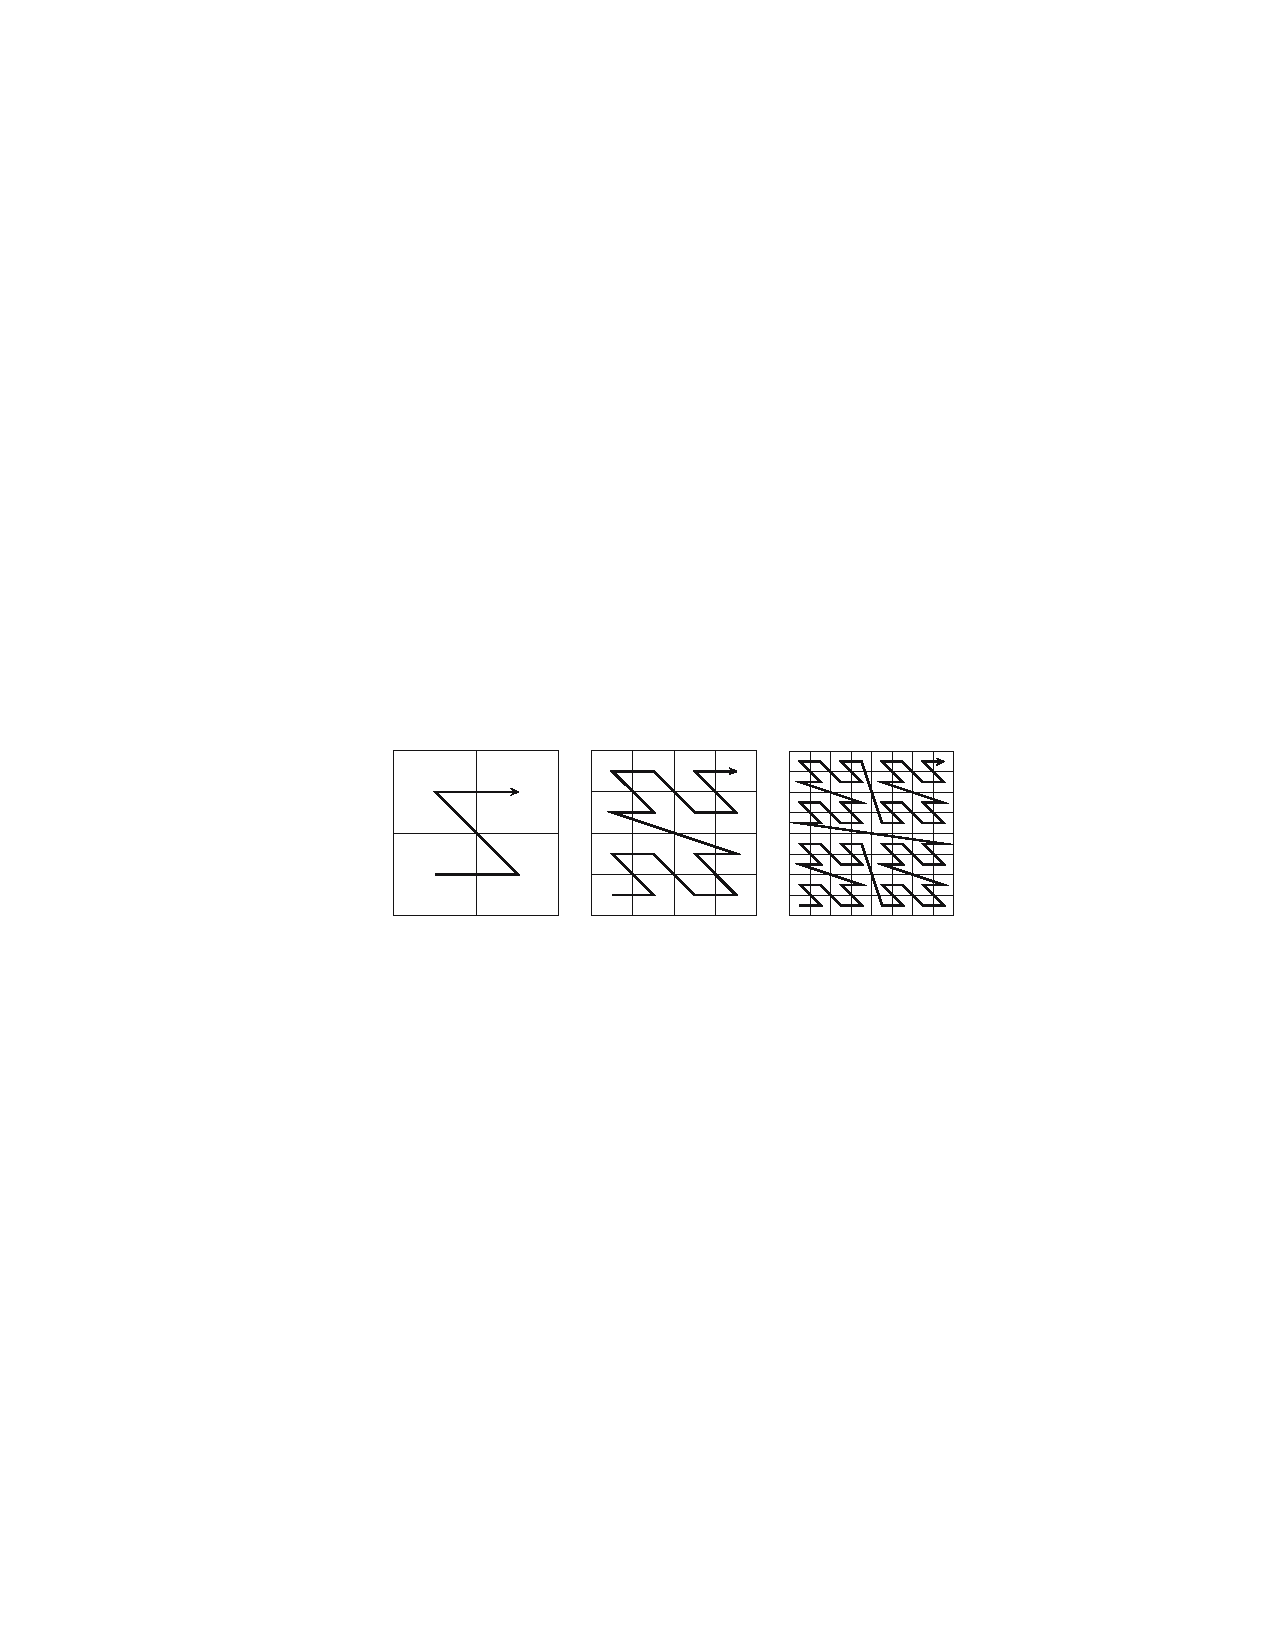
\includegraphics[scale=1.0, viewport = 150 350 500 435, clip]{figures/lebesgue.pdf}
    \caption{\footnotesize{Three refinement levels in the construction of the Lebesgue 
	curve in 2D.}}
    \label{fig:lebesgue}
\end{figure}
\begin{figure}[ht]
    \centering
    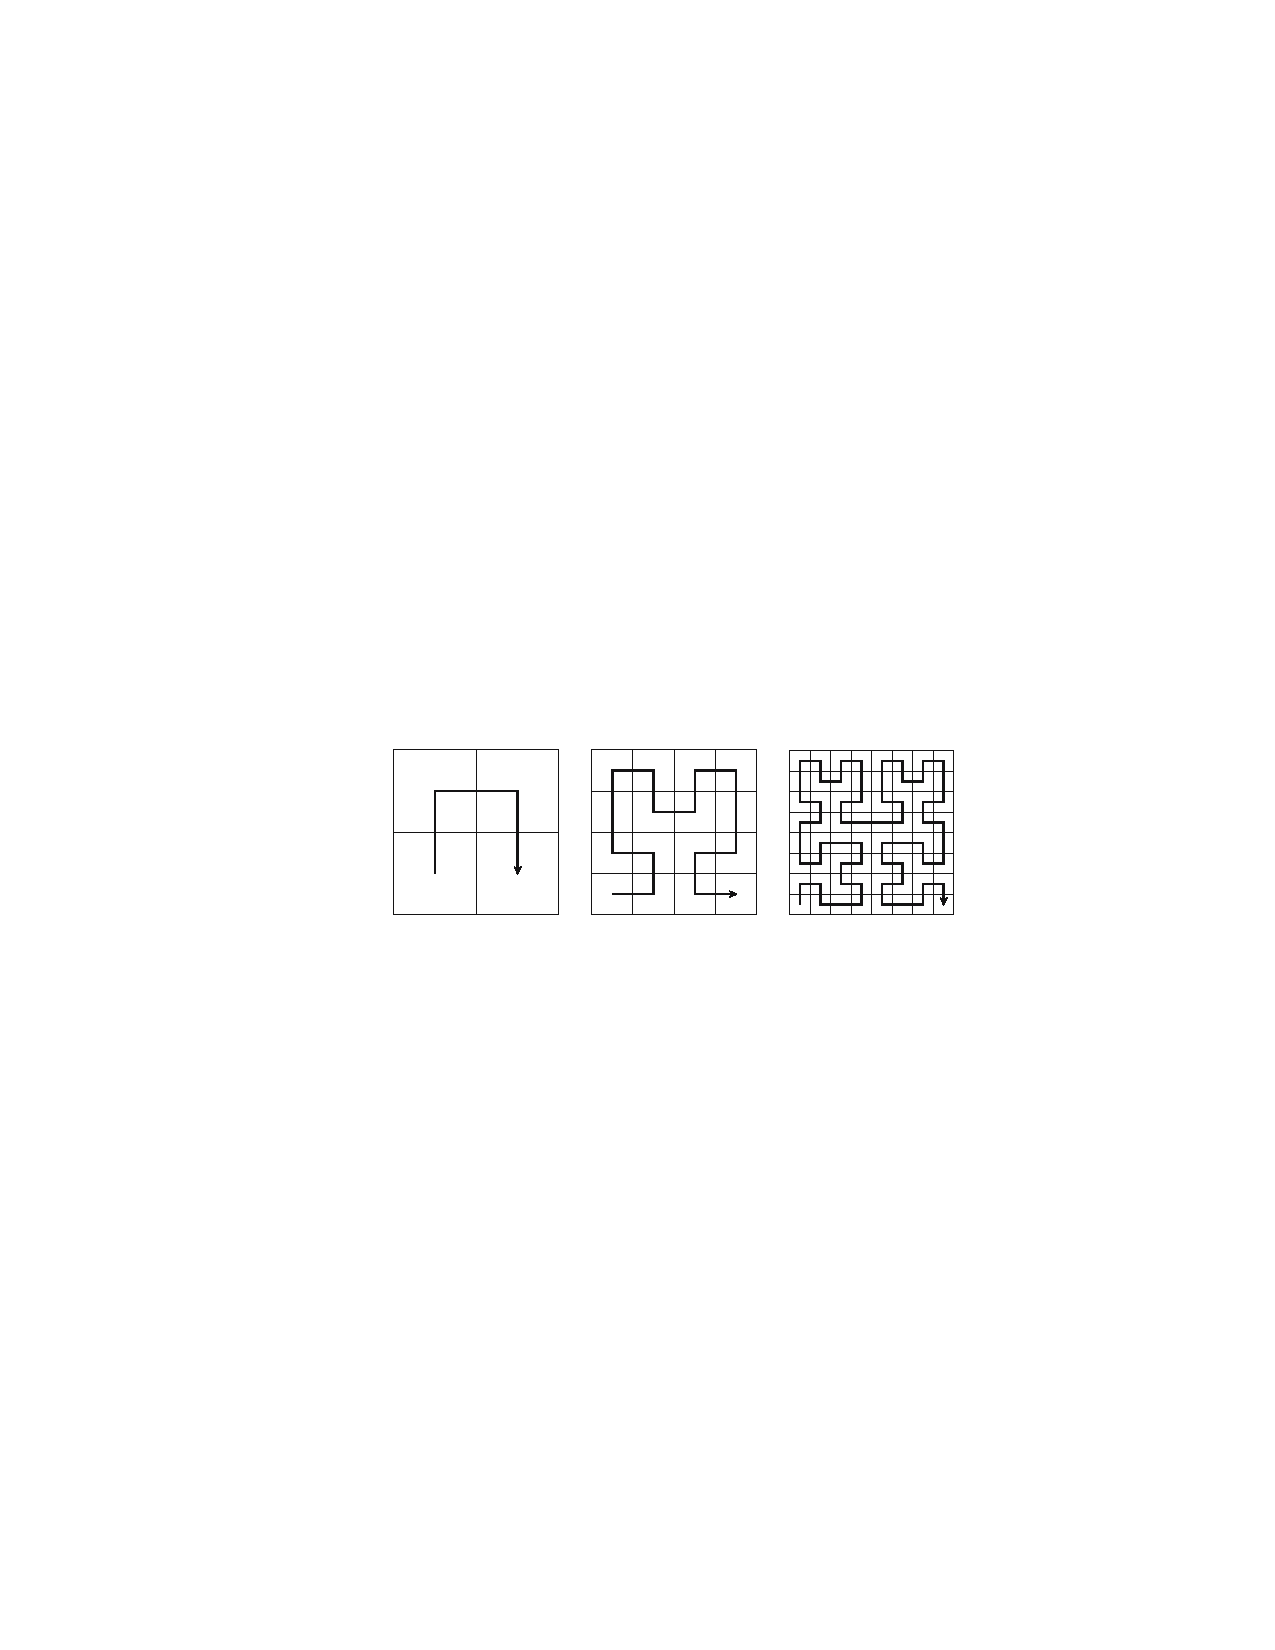
\includegraphics[scale=1.0, viewport = 150 350 500 435, clip]{figures/hilbert.pdf}
    \caption{\footnotesize{Three refinement levels in the construction of the Hilbert 
	curve in 2D.}}
    \label{fig:hilbert}
\end{figure}

There are several possible strategies for how the \nodes could be distributed
and we have chosen one that leads to strictly connected domains, in the sense 
that all \nodes belonging to a given host is connected (share a common vertice,
not necessarily on the same scale) to at least one other \node owned by the same 
host. This ensures that the real-space domain of a given host will be localized 
in space, with the motivation that the interaction between hosts could be limited
to involve only near neighbors, and thus hopefully reduce the need for communication
between hosts.

In order to achieve this localization we traverse the \tree following a space-filling
path, assigning \nodes to hosts as we go. By following a so-called Hilbert 
path~\cite{Griebel:2007}, we obtain a continuous curve with good locality properties, 
that can be partitioned among the hosts. The construction of the curve is done 
recursively, going through the $2^d$ children of each \node in a specific order. 
Using bit notation (one bit for each dimension), the natural ordering (Lebesgue) will 
lead to a discontinuous path. For $d=2$ this is shown as the Z shape of the bit sequence 
(00, 01, 10, 11) in figure \ref{fig:lebesgue}. A corresponding (there are several 
possibilities) Hilbert path through the four children in two dimensions could be the 
bit sequence (00, 10, 11, 01) shown in the first panel in figure \ref{fig:hilbert}. 
In order to keep the continuouity as the path is recursively refined, the order in 
which the children are traversed needs to be adapted, and will depend on the position 
of the parent among its siblings, as shown in figure \ref{fig:hilbert}.

\section{Adaptive algorithm}
\begin{algorithm}
    \footnotesize
    \caption{Generation of adaptive multiwavelet representation of a function}
    \label{alg:function}
    \begin{algorithmic}[1]
	\STATE create \tree skeleton of empty \nodes
	\STATE MPI: distribute leaf \nodes among hosts through Hilbert path
	\STATE MPI: create list of local \nodes owned by \emph{this} host
	\WHILE{number of local \nodes on current iteration $N_i>0$}
	    \STATE OpenMP: divide local \nodes among available processors
	    \FOR{each \node at current iteration}
		\STATE compute scaling and wavelet coefficients
		\IF{\node needs to be refined}
		    \STATE mark \node as non-terminal
		    \STATE allocate children \nodes
		    \STATE update list of local \nodes for next iteration
		\ELSE
		    \STATE mark \node as terminal
		\ENDIF
	    \ENDFOR
	    \STATE increment iteration
	\ENDWHILE
    \end{algorithmic}
\end{algorithm}

\noindent
Algorithm \ref{alg:function} used to obtain adaptive representations of functions 
was originally presented in \cite{Frediani:2013p1143}, but is here extended to 
include parallelization. The first lines in this algorithm are very important in 
order to ensure a good
load balancing among MPI hosts. By utilizing some a priori knowledge of the
function that is about to be buildt, we try to estimate the final \tree structure
as closely as possible before calculating any coefficients. In this way we have
a lot more flexibility when it comes to parallel distribution of data and work load 
in all iterations. Without this preprocessing step, the first three iterations would 
contain one, eight and 64 \texttt{nodes}, respectively, allowing little freedom in
parallel computations. It is important in this step to capture the global structure
of the function (where in space is high level of refinement needed), as this initial
\tree skeleton is used in the data distribution among MPI hosts and all subsequent
additional refinent is done locally on each host (although some load balancing can
be preformed by redistribution of data if needed). How to construct this skeleton
depends on the function, and will be discussed in the following sections.

The algorithm consists of two loops, the first iteration will add levels of 
refinement on top of the initial skeleton wherever necessary in order to guarantee
the overall accuracy of the representation. This loop terminates when no further
refinement is needed. The second loop runs over the \nodes present at the current 
iteration (only local \nodes that belong to the given MPI host), and these are 
distributed among the available processors (OpenMP) at the given host. Once the 
scaling/wavelet coefficients of a given \node are known, a split check is performed 
based on the desired precision. If the \node does not satisfy the accuracy criterion, 
it is marked as non-terminal and its children \nodes are allocated and added to the 
list of \nodes needed in the next iteration. If the \node does not need to be split, 
it is marked as terminal and no children \nodes are allocated. In this way, once the 
loop over \nodes on one iteration is terminated, the complete list of \nodes needed 
in the next iteration has been obtained. The \tree is grown until no \nodes are 
needed at the next iteration.

There are two points in the algorithm that need to be elaborated further, the first 
being the actual computation of the coefficients (line 7). This can be done in 
many ways, e.g. projection or by operator application, and will be treated in 
the subsequent sections. 

The second point is how to perform the split check (line 8), which is used to decide 
whether or not the function is represented accurately enough on the current 
\texttt{node}, based on a predefined relative precision $\epsilon$. Formally, this 
relative precision requires that 
\begin{equation}
    \|f-\scalingrep{f}{n}\| < \epsilon \|f\|
\end{equation}
However, this check cannot be performed since the \emph{true} function $f$ is 
generally not known. Instead we will use the norm of the wavelet projections as a
measure of the accuracy of the representation. Specifically, the norm of the wavelet 
coefficients on one \node is used as a measure for the accuracy of the part of the
function represented by this \texttt{node}, and we require that
\begin{equation}
    \|\bs{\waveletcoef}^n_{\bs{l}}\| < \frac{\epsilon}{2^{n/2}} \|\scalingrep{f}{n}\|
\end{equation}
The local, disjoint support of the wavelet basis ensures that the global error of
the representation can be controlled by locally truncating the wavelet expansion,
allowing a fully on-the-fly adaptive algorithm. This reduces the number of expansion 
coefficients needed to represent the function to the given accuracy dramatically 
compared to the uniform high-resolution representation in Eq.~(\ref{eq:highres}).
In practical calculations one can easily get significant contribution over a range
of ten length scales, and a uniform grid in three dimensions at scale $n=10$ would
require $(2^d)^n = 8^{10} \sim 10^9$ \texttt{nodes}, while a typical multi-resolution
representation requires in the order of $10^2-10^4$ \nodes per scale. Figure 
\ref{fig:adapgrid} shows the grid needed to represent a spherical Gaussian
positioned at the center of the unit cube.

The presented algorithm is very general, and is used to build adaptive 
representations of functions regardless of how the expansion coefficients are 
obtained, and later in the chapter we will look at different ways of doing this.

\begin{figure}
    \centering
    \includegraphics[scale=0.5]{figures/adapgrid.pdf}
    \caption{\footnotesize{Adaptive grid-partitioning of the unit cube needed to
    reproduce the Gaussian function
    $f(\bs{x}) = (\beta/\pi)^{3/2} e^{-\beta(\bs{x}-\bs{x}_0)^2}$ with exponent 
    $\beta=500$ in position $\bs{x}_0 = (1/2,1/2,1/2)$ to a relative accuracy of 
    $\epsilon = 10^{-8}$ using multiwavelets of order $k=9$.}}
    \label{fig:adapgrid}
\end{figure}

\section{Choice of basis functions}
Before we can describe how to calculate expansion coefficients we need to specify
the type of scaling and wavelet functions that is used in the multiresolution 
analysis. In principal, any polynomial basis that span the appropriate scaling
\scalingspace{n} and wavelet \waveletspace{n} spaces can be used, and in the original 
construction Alpert~\cite{Alpert:1993p5460} used Legendre polynomials as scaling basis, 
but in a later work, Alpert \etal~\cite{Alpert:2002p149} introduced an alternative 
basis with interpolating properties. Both scaling bases have been implemented, but 
in practice only the latter is used, because of its superior numerical efficiency. 
The choice of wavelet basis follows that of Alpert~\cite{Alpert:1993p5460}.

\subsection{Legendre scaling functions}
The Legendre polynomials $\lbrace L_j(x)\rbrace_{j\in \mathbb{N}}$ are a family of 
functions, defined on the interval $[-1,1]$. The functions are orthogonal with 
respect to the $L^2([-1,1])$ inner product
\begin{equation}
    \int_{-1}^{1} L_i(x)L_j(x) \ud x = 0, \qquad i \neq j
\end{equation}
but they are usually normalized such that $L_j(1) = 1$. The polynomials can be 
constructed by induction
\begin{align}
    L_0(x) &= 1\\
    L_1(x) &= x\\
    L_{j+1}(x) &= \frac{2j+1}{j+1}xL_j(x) - \frac{j}{j+1}L_{j-1}
\end{align}
and the \emph{Legendre scaling functions} $\scaling_j^L$ are obtained by dilation 
and translation to the unit interval, followed by $L^2$ normalization
\begin{equation}
    \scaling_j^L(x) = \sqrt{2j+1}L_j(2x-1),\qquad x \in [0,1]
\end{equation}
This is the original construction of scaling functions by 
Alpert~\cite{Alpert:1993p5460}.

\subsection{Interpolating scaling functions}
Alpert \etal~\cite{Alpert:2002p149} presented an alternative set of scaling functions 
with interpolating properties. These \emph{Interpolating scaling functions} 
$\scaling_j^I$ are based on the Legendre scaling functions $\lbrace \scaling_j^L
\rbrace_{j=0}^k$, and the roots $\lbrace x_j\rbrace_{j=0}^k$ and weights
$\lbrace \omega_j \rbrace_{j=0}^k$ of the Gauss-Legendre quadrature of order 
$k+1$, and are constructed as the linear combinations
\begin{equation}
    \label{eq:interpolating}
    \scaling_j^I(x) = \sqrt{\omega_j}\sum_{i=0}^{k} 
	\scaling_i^L(x_j)\scaling_i^L(x),\qquad x \in [0,1]
\end{equation}
This construction leads to orthogonality on the unit interval, as well as the 
interpolating property
\begin{equation}
    \label{eq:interprop}
    \scaling_j^I(x_i) = \frac{\delta_{j,i}}{\sqrt{\omega_i}}
\end{equation}
which will prove important for numerical efficiency. A detailed discussion on 
the properties of Interpolating wavelets can be found in Donoho~\cite{Donoho:1992}.

\subsection{Wavelet basis}
There are two necessary constraints in the construction of the wavelet functions
$\wavelet_j$: they must be orthogonal to the scaling functions and orthogonal among 
themselves. It turns out that this is not sufficient to determine the wavelet functions
uniquely, so Alpert~\cite{Alpert:1993p5460} posed additional conditions in terms of 
vanishing moments. The exact construction is done iteratively, starting with the 
following set of functions $\lbrace f_j(x) \rbrace_{j=0}^k$ defined on the interval 
$(-1,1)$

\begin{equation}
    f_j(x) = 
    \left\{
	\begin{array}{lll}
	    x^j,	& x \in (0,1)\\
	    -x^j,	& x \in (-1,0)\\
	    0,		& otherwise
	\end{array}
    \right.
\end{equation}
\ \\
\noindent
followed by a Gram-Schmidt orthogonalization with respect to the low-order polynomials
$1,x,x^2,\dots,x^k$ that span the corresponding scaling space. Furthermore, we require
that the function $f_j$ has $j+1$ additional vanishing moments by orthogonalization 
with respect to the polynomials $x^{k+1},\dots,x^{j+k+1}$, and finally, the functions
$f_j$ are orthogonalized among themselves in order of increasing $j$. The wavelet basis 
$\wavelet_j$ of the space \waveletspace{0} is then constructed by dilation and 
translation to the unit interval, followed by $L^2$ normalization.

\section{Function projection}\label{sec:impl_func_proj}
In order to obtain the expansion coefficients of a general function $f$ in the 
scaling basis we need to evaluate the projection integral in 
Eq.~(\ref{eq:scaling_exp}). This is done numerically using Gauss-Legendre quadrature
\begin{align}
    \scalingcoef_{j,l}^{n,f} 
	&= \int_{2^{-n}l}^{2^{-n}(l+1)} f(x)\scaling_{j,l}^n(x)\ud x\\
	&= 2^{-n/2}\int_0^1 f\big(2^{-n}(x+l)\big) \scaling_j(x)\ud x\\
	\label{eq:quadrature}
	&\approx 2^{-n/2}\sum_{q=0}^{k_q-1} \omega_q f\big(2^{-n}(x_q+l)\big) 
	    \scaling_j(x_q)
\end{align}
where $\lbrace \omega_q\rbrace_{q=0}^{k_q-1}$ are the weights and
$\lbrace x_q\rbrace_{q=0}^{k_q-1}$ the roots of the Legendre polynomial $L_{k_q}$ 
used in $k_q$-th order quadrature. The Legendre quadrature holds a $(2k-1)$-rule 
which states that the $k$-order quadrature is exact whenever the integrand is a 
polynomial of order $2k-1$. By choosing $k_q = k+1$ order quadrature, where $k$ is
the order of the polynomial basis, we will obtain the exact coefficient
whenever $f(x)$ is a polynomial of degree $\leq (k+1)$, and we will use quadrature 
order $k+1$ throughout.

\subsection{Projection in $d$ dimensions}
In the multi-dimensional case the expansion coefficients are given by
multi-dimensional quadrature
\begin{equation}
    \label{eq:multidimprojection}
    \scalingcoef^{n,f}_{\bs{j},\bs{l}} = 2^{-nd/2}
	\sum_{q_1=0}^{k}\sum_{q_2=0}^{k}\cdots\sum_{q_d=0}^{k}
        f\big(2^{-n}(\bs{x_q}+\bs{l})\big)
	\prod_{i=1}^d \omega_{q_i}\scaling_{j_p}(x_{q_i})
\end{equation}
using the following notation for the vector of quadrature roots
\begin{align}
    \bs{x_q} &\mydef (x_{q_1},x_{q_2},\dots,x_{q_d})
\end{align}
This multi-dimensional quadrature is not very efficient in a general polynomial 
basis, as the number of terms scales as $(k+1)^d$. This can be avoided if the 
function $f$ is separable and can be written $f(x_1,x_2,\dots,x_d) = 
f_1(x_1)f_2(x_2)\cdots f_d(x_d)$, in which Eq.~(\ref{eq:multidimprojection}) can be 
reduced to a product of mono-dimensional summations with a scaling of $d(k+1)$.

However, working in the Interpolating basis, no assumption needs to be made on
the function to obtain numerical efficiency. By choosing a quadrature order of 
$k_q=k+1$, a very important property of the Interpolating scaling functions 
emerges, that follows from the specific construction of these functions in 
Eq.~(\ref{eq:interpolating}). 
The interpolating property in Eq.~(\ref{eq:interprop}) inserts a Kronecker delta 
whenever the scaling function is evaluated in a quadrature root, which is exactly the 
case in the quadrature sum. This reduces Eq.~(\ref{eq:multidimprojection}) to
\begin{equation}
    \label{eq:inter_quad}
    \scalingcoef^{n,f}_{\bs{j},\bs{l}} = 2^{-nd/2}
	f\big(2^{-n}(\bs{x_j}+\bs{l})\big)\prod_{i=1}^d \sqrt{\omega_{j_i}}
\end{equation}
which means that the scaling coefficients are related by simple constant factors to 
the function values on the quadrature grid, leading to very efficient evaluation.

\subsection{Obtaining the wavelet coefficients}
The wavelet coefficients are formally obtained by the projection of the
function onto the wavelet basis, and we could derive expressions similar to
the scaling expressions based on quadrature. There are however some accuracy
issues connected to this wavelet quadrature, so we will take another approach 
that utilizes the wavelet transform. We know that we can obtain the scaling and
wavelet coefficients on scale $n$ by doing a wavelet decomposition of the
scaling coefficients on scale $n+1$ according to Eq.~(\ref{eq:twoscalerelations}).
Line 7 of algorithm \ref{alg:function} is thus performed by computing the scaling
coefficients of the $2^d$ children of the current \node by the appropriate 
expression (Legendre or Interpolating) followed by a wavelet decomposition. 

\subsection{Estimating the \tree structure}
In projection of analytic functions it is quite straightforward to predict the
final adaptive \tree structure of the representation without any actual calculation
of coefficients. E.g. in the case of Gaussian ($e^{-\beta (\bs{x}-\bs{x}_0)^2)}$) 
and Slater ($e^{-\beta |\bs{x}-\bs{x}_0|}$) type functions, the position $\bs{x}_0$ 
and exponent $\beta$
tells you where and approximately how much the grid needs to be refined. Furthermore, 
in the case of very narrow, high-exponent functions this "forced" refinement is
essential, as the quadrature at the coarsest scale would probably not pick up
any signal at all, leaving you with a zero-representation of the function.

\section{Arithmetic operations}
\subsection{Addition}
The recipe for the addition of two function \trees follows straightforwardly
from the mappings in Eq.~(\ref{eq:addmap}). Consider the equation $h(x) = f(x)+g(x)$. 
Projecting $h$ onto the scaling space \scalingspace{n} yields
\begin{align}
    h^n(x)  &= \scalingproj{n}\left(f(x)+g(x)\right)\\
	    &= \scalingproj{n}f(x)+\scalingproj{n}g(x)\\
    \label{eq:scalingadd}
	    &= \scalingrep{f}{n}(x)+\scalingrep{g}{n}(x)
\end{align}
and similarly for the wavelet projections. At a deeper level it simply means adding 
scaling and wavelet coefficients on corresponding \nodes
\begin{align}
    \scalingcoef^{n,h}_{j,l} 
	&= \scalingcoef^{n,f}_{j,l}+\scalingcoef^{n,g}_{j,l}\\
    \waveletcoef^{n,h}_{j,l}
	&= \waveletcoef^{n,f}_{j,l}+\waveletcoef^{n,g}_{j,l}
\end{align}
If the given \node does not exist in the representation of either $f$ or $g$, it is 
obtained by oversampling using the wavelet transform Eq.~(\ref{eq:twoscalerelations}). 
No absolute accuracy will be lost during an addition, but \emph{relative} 
accuracy might be lost if the additon reduces the norm of the function.

\subsection{Multiplication}
Consider the equation $h(x) = f(x)\times g(x)$. In practice this means to
multiply the representations \scalingrep{f}{n} and \scalingrep{g}{n}
\begin{equation}
    \label{eq:multiplication}
    h(x) \approx \hat{h}(x) \mydef \scalingrep{f}{n}(x) 
	\times \scalingrep{g}{n}(x)\\
\end{equation}
However, as we have seen in section \ref{sec:multiplication}, the product of the
scaling representations at scale $n$ will give wavelet contributions at higher
scales, and Beylkin~\cite{Beylkin:1992}
suggests to perform the multiplication of \emph{oversampled} function representations 
\begin{equation}
    \scalingrep{\hat{h}}{n+1}\ =\ \ \scalingproj{n+1}\Big( 
	\uparrow(\scalingrep{f}{n})\ \times\ \uparrow(\scalingrep{g}{n}) \Big)
\end{equation}
to allow enough flexibility in the basis to represent the product. In our 
implementation the adaptive algorithm will take care of the extra refinement in the 
product only if and where it is necessary. We will thus perform the multiplication 
in Eq.~(\ref{eq:multiplication}) purely on the given scale $n$, which means that we
project the product of the representations back onto the scaling space 
\scalingspace{n}
\begin{equation}
    \scalingrep{\hat{h}}{n} = 
	\scalingproj{n}\big(\scalingrep{f}{n} \times \scalingrep{g}{n}\big)
\end{equation}
and the coefficients of the product are approximated by the projection integral
\begin{align}
    \scalingcoef^{n,h}_{j^h,l} 
	&\approx \int_{2^{-n}l}^{2^{-n}(l+1)}
	    \hat{h}(x)\scaling_{j^h,l}^n(x)\ud x\\
	&= \int_{2^{-n}l}^{2^{-n}(l+1)}
	    \scalingrep{f}{n}(x)\scalingrep{g}{n}(x)\scaling^n_{j^h,l}(x)\ud x\\
	&= 2^{-n/2} \int_0^1
	    \scalingrep{f}{n}\big(2^{-n}(x+l)\big)
	    \scalingrep{g}{n}\big(2^{-n}(x+l)\big)\scaling_{j^h}(x)\ud x
    \label{eq:multexpansion}
\end{align}
The projection integral is again done by Gauss-Legendre quadrature and all the 
information we need from the multiplicands are their pointvalues in the quadrature 
roots $\lbrace x_q\rbrace_{q=0}^k$ at scale $n$, which can be obtained from their
respective scaling coefficients
\begin{align}
    \scalingcoef^{n,h}_{j^h,l} &\approx 2^{-n/2}
	\sum_{q=0}^k \omega_q \scalingrep{f}{n}\big(2^{-n}(x_q+l)\big)
        \scalingrep{g}{n}\big(2^{-n}(x_q+l)\big) \scaling_{j^h}(x_q)\\
	&= 2^{n/2}\sum_{q=0}^k \omega_q 
	\left(\sum_{j^f=0}^k\scalingcoef^{n,f}_{j^f,l}\scaling_{j^f}(x_q)\right)
	\left(\sum_{j^g=0}^k\scalingcoef^{n,g}_{j^g,l}\scaling_{j^g}(x_q)\right)
	\scaling_{j^h}(x_q)
	\label{eq:nmult}
\end{align}

\subsection{Multiplication in $d$ dimensions}
Generalizing the above expression for multiple dimensions reveals that multiplication
will become a time consuming process in a general polynomial basis
\begin{align}
    \label{eq:legmultND}
    \begin{split}
    \scalingcoef^{n,h}_{\bs{j}^h,\bs{l}} 
	\approx&\ 2^{nd/2} 
	\sum_{q_1=0}^k\sum_{q_2=0}^k\cdots\sum_{q_d=0}^k\Bigg(
	\bigg(\prod_{i=1}^d\omega_{q_i}\bigg)\\
	&\ \ \times\Bigg(\sum_{j^f_1=0}^k\sum_{j^f_2=0}^k\cdots\sum_{j^f_d=0}^k
	\scalingcoef^{n,f}_{\bs{j}^f\bs{l}} \bigg(
	\prod_{i=1}^d\scaling_{j^f_i}(x_{q_i})\bigg)\Bigg)\\
	&\ \ \times\Bigg(\sum_{j^g_1=0}^k\sum_{j^g_2=0}^k\cdots\sum_{j^g_d=0}^k
	\scalingcoef^{n,g}_{\bs{j}^g\bs{l}} \bigg(
	\prod_{i=1}^d\scaling_{j^g_i}(x_{q_i})\bigg)\Bigg)\\
	&\ \ \times \ \ \ 
	\prod_{i=1}^d\scaling_{j^h_i}(x_{q_i})\Bigg)
    \end{split}
\end{align}
The scaling behavior of this expression is $(k+1)^{2d}$, however, the only function 
evaluations that are actually taking place are again the $k+1$ different scaling 
functions evaluated in the $k+1$ different quadrature roots. These $(k+1)^2$ function
values need to be evaluated only once, and fetched from memory whenever needed in 
the expression Eq.~(\ref{eq:legmultND}), which will speed up the process.

Working in the Interpolating basis, the multiplication complexity is significantly 
reduced, as the basis is specifically designed to return Kronecker deltas when 
evaluated in the quadrature roots. Inserting this property in 
Eq.~(\ref{eq:legmultND}), all nested summations are removed and we are left with a 
single term in the evaluation of the coefficient of the product 
\begin{equation}
    \scalingcoef^{n,h}_{\bs{j}^h\bs{l}} =\ 2^{nd/2}
	\scalingcoef^{n,f}_{\bs{j}^h\bs{l}}
	\scalingcoef^{n,g}_{\bs{j}^h\bs{l}}
	\prod_{i=1}^d\frac{1}{\sqrt{\omega_{j^h_i}}}
	\label{eq:intmultND}
\end{equation}

\subsection{Obtaining the wavelet coefficients}
In the case of multiplication, the calculation of the wavelet coefficients on
a given scale $n$ is done in the same way as for the
projection, by wavelet transform of the scaling coefficients at scale $n+1$.
Line 7 of algorithm \ref{alg:function} is again obtained by calculation of the 
scaling coefficients of the $2^d$ children of the current \node by the
appropriate expression (Legendre or Interpolating), followed by a wavelet
decomposition.

\subsection{Estimating the \tree structure}
In both addition and multiplication we use the union of the \tree structures of
the input functions as the starting guess for the \tree structure of the result.
In the case of addition, there is no need for further refinement, as there will 
be no wavelet contribution beyond this level of refinement in the result. In 
multiplications, however, it might be necessary to refine a scale or two locally,
and this is taken care of by the adaptive algorithm.

\section{Operator construction}
It was shown in chapter \ref{chap:mathematics} that the matrix elements of a general
one-dimensional integral operator is obtained by projection of the two-dimensional
integral kernel onto the multiwavelet basis. This corresponds to a regular function
projection, as described in section \ref{sec:impl_func_proj}, and at the end of the 
day the construction of such operators will follow the algorithms presented above for
projection. However, for $d$-dimensional problems, the integral kernel will in general
have $2d$ dimensions, and this complexity needs to be reduced in order to obtain
efficient algorithms both in the construction and application of operators in multiple
dimensions. This can be achieved by the technique of separation of variables.

\subsection{Separated representation of operators}
In the discussion of multi-dimensional operators in chapter \ref{chap:mathematics} it
was assumed that the kernel is separable in the Cartesian coordinates. This assumption 
is necessary in order to make calculations feasable in higher dimensions, as the 
straightforward generalization of a one-dimensional approach leads to a prohibitive 
exponential scaling in the dimension. It is,
however, not necessary that the operator separates exactly, and Beylkin 
and Mohlenkamp~\cite{Beylkin:2002p429,Beylkin:2005p45} shows that the integral 
kernel of many physically interresting operators can be approximated as a linear 
combination of products of one-dimensional kernels
\begin{equation}
    \label{eq:sep_rep}
    K(\bs{x},\bs{y}) \approx \hat{K}(\bs{x},\bs{y}) \mydef 
	\sum_{\kappa=1}^{M}\alpha_\kappa \prod_{p=1}^d K_p^\kappa(x_p,y_p)
\end{equation}
The accuracy of this separated representation can be controlled by adapting
the functions $K_p^\kappa$, the expansion coefficients $\alpha_\kappa$ and the 
separation rank $M$, and any precision can in principle be achieved. Such
a representation allows the multi-dimensional operator to be applied one 
dimension at the time, reducing the computational complexity from
$k^{2d}$ per \node of the full non-separable operator, to $Mdk^{d+1}$ 
per \node of the separated representation in Eq.~(\ref{eq:sep_rep}),
where $k$ is the order of the polynomial basis. While the scaling is still 
exponential in the dimension, the exponent is sufficiently reduced for the 
approach to be applicable for $d=2,3$. 

\subsection{Poisson kernel}
The Poisson equation is usually written in its differential form
\begin{equation}
    \nabla^2 g(\bs{x}) = -f(\bs{x})
\end{equation}
and the solution of can be expressed in terms of the convolution integral
\begin{equation}
    g(\bs{x}) = \int P(\bs{x}-\bs{y})f(\bs{y})\ud\bs{y}
\end{equation}
where $P(\bs{x}-\bs{y})$ is the Green's function satisfying the fundamental 
equation with free boundary conditions (zero at infinity)
\begin{equation}
    \label{eq:fundamental_poisson}
    \nabla^2 P(\bs{x}-\bs{y}) = -\delta(\bs{x}-\bs{y})
\end{equation}
This equation can be solved analytically and the Green's function for
the Poisson equation for $d=3$ is given as
\begin{equation}
    \label{eq:poisson_kern}
    P(\bs{x}-\bs{y}) = \frac{1}{4\pi||\bs{x}-\bs{y}||}
\end{equation}

\subsection{Helmholtz kernel}
The inhomogeneous Helmholtz equation is a generalization of the Poisson equation,
and is given in differential form
\begin{equation}
    \big(\nabla^2 + \mu^2\big) g(\bs{x}) = -f(\bs{x})
\end{equation}
The solution can again be expressed as an integral
\begin{equation}
    g(\bs{x}) = \int H^\mu(\bs{x}-\bs{y})f(\bs{y})\ud\bs{y}
\end{equation}
using the Helmholtz kernel $H^\mu(\bs{x}-\bs{y})$, which is the Greeen's function 
satisfying the fundamental equation
\begin{equation}
    \label{eq:fundamental_helmholtz}
    \big(\nabla^2 + \mu^2\big) H^\mu(\bs{x}-\bs{y}) = -\delta(\bs{x}-\bs{y})
\end{equation}
with zero boundary conditions at infinity. The Green's function for the Helmholtz 
equation for $d=3$ is known analytically as
\begin{equation}
    \label{eq:helmholtz_kern}
    H^\mu(\bs{x}-\bs{y}) = \frac{e^{-\mu\|\bs{x}-\bs{y}\|}}{4\pi||\bs{x}-\bs{y}||}
\end{equation}

\subsection{Separation using Gaussians}
Neither the Poisson nor Helmholtz kernels are separable in the Cartesian coordinates, 
but it is possible to obtain a separated representation as in Eq.~(\ref{eq:sep_rep}) 
of low rank using Gaussian functions
\begin{equation}
    \label{eq:gaussian_exp}
    K(\bs{x}-\bs{y}) \approx \hat{K}(\bs{x}-\bs{y}) = 
	\sum_{\kappa=1}^M \alpha_\kappa e^{-\beta_\kappa \|\bs{x}-\bs{y}\|^2}
\end{equation}
This representation is motivated by the well known integral representation of the 
Poisson kernel\cite{Singer:1960}
\begin{equation}
    \label{eq:poisson_int_rep}
    P(r) = \frac{1}{r} = \frac{4}{\sqrt{\pi}}\int_0^\infty e^{-4r^2t^2}\ud t, 
	\quad r \mydef \|\bs{x}-\bs{y}\|
\end{equation}
and the parameters in Eq.~(\ref{eq:gaussian_exp}) are obtained in the case of the 
Poisson kernel by transforming Eq.~(\ref{eq:poisson_int_rep}) into an integral of 
super-exponential decay, and discretizing using the trapezoidal 
rule~\cite{Harrison:2003,Frediani:2013p1143}. In this way, 
and similarly in the case of the Helmholtz kernel, it is possible to obtain a separated 
representation $\hat{K}$ of Eq.(\ref{eq:gaussian_exp}) with accuracy $\epsilon_s$ over a 
finite interval
\begin{equation}
    sup_{r>0}\Big|\frac{K(r)-\hat{K}(r)}{K(r)}\Big| < \epsilon_s, \quad r\in[r_0,r_1]
\end{equation}
where the upper bound $r_1$ should be chosen as the longest possible distance
in the computational domain ($r_1=\sqrt{3}$ for the unit cube), and the lower
bound $r_0$ should be chosen so that the contribution due to the integration
at the singularity can be neglected\cite{Frediani:2013p1143}.

\subsection{Derivative kernel}
As a final note we show how we can obtain approximate representations of the 
derivative operator using the framework of integral operators presented above. 
The derivative operator can be expressed as
\begin{equation}
    \frac{\ud}{\ud x} f(x) = \int \frac{\ud}{\ud x} \delta(x-y) f(y) \ud y
\end{equation}
where the delta function can be approximated by a high-exponent Gaussian
\begin{equation}
    \label{eq:delta_approx}
    \delta(x-y) \approx \sqrt{\frac{\beta}{\pi}} e^{-\beta (x-y)^2}
\end{equation}
which is normalized so that it integrates to unity. This approximation can be 
differentiated, and the derivative operator can be expressed as the integral
\begin{equation}
    \frac{\ud}{\ud x} f(x) = \int D(x-y)f(y) \ud y
\end{equation}
using the derivative kernel
\begin{equation}
    D(x-y)  = \frac{\ud}{\ud x} \sqrt{\frac{\beta}{\pi}}e^{-\beta (x-y)^2} 
	    = -2\beta \sqrt{\frac{\beta}{\pi}}(x-y)e^{-\beta (x-y)^2}
\end{equation}
This representation approaches the exact derivative as defined by Alpert 
\etal~\cite{Alpert:2002p149} and presented in section \ref{sec:diff_oper} as 
the Gaussian in Eq.~(\ref{eq:delta_approx}) approaches the delta function 
($\beta \rightarrow \infty$).

\subsection{Cross-Correlation functions}
All operators presented above involve integrals with convolution kernels
$K(x,y) = K(x-y)$, and the matrix elements can be expressed in terms of the
cross-correlation of the scaling functions~\cite{Fann:2004}
\begin{equation}
    \Phi_{ij}(z) = \int_0^1 \phi_i(z+y)\phi_j(y) \ud y
\end{equation}
and the two-dimensional projection integral is reduced to one dimension
\begin{align}
    \big[\tau_{lm}^n\big]_{ij}
	&= \int_0^1 \int_0^1 K(x-y)\phi_i^n(x-l)\phi_j^n(y-m) \ud x \ud y \\
	&= \int_{-1}^1 K(z)\Phi_{ij}(2^nz+m-l)\ud z
\end{align}
For $d$-dimensional operators the kernel is $2d$-dimensional, and the cross-correlation 
functions will reduce the integral to $d$ dimensions. Moreover, if the kernel is
separable, the matrix element can be computed as products of one-dimensional integrals
\begin{equation}
    \big[\tau_{\bs{l}\bs{m}}^n\big]_{ij} = \prod_{p=1}^d\int_{-1}^1 
	K_p(z_p)\Phi_{ij}\big(2^nz_p+m_p-l_p\big) \ud z_p
\end{equation}
which significantly reduces the cost of constructing multi-dimensional operators. 

\section{Operator application}
In the non-standard operator application given in the matrix 
equation~(\ref{eq:NSmatrix}), the length scales of the problem have been
explicitly separated. In this way it is possible to use 
algorithm~\ref{alg:function} to adaptively build the resulting function \texttt{tree}, 
also in several dimensions. For a \node at a given scale $n$ we need to calculate 
the scaling and wavelet representations of the resulting function $g$
\begin{equation}
    \label{eq:oper_n}
    \scalingrep{g}{n} + \waveletrep{g}{n} = 
	\big(\ \A{n}{n}\ +\ \B{n}{n}\ +\ \C{n}{n}\ +\ \T{n}{n}\ \big)
	\big(\scalingrep{f}{n} + \waveletrep{f}{n}\big)
\end{equation}
but as was pointed out in the theory part in section~\ref{sec:operator}, the
$T$ part of the operator is only applied at the coarsest scale, and thus, no
interaction with the coarser scales are taken into account for $n>0$. However,
when the operator is applied scale by scale, the effect of the missing $T$ part
at scale $n$ has already been calculated at scale $n-1$, and this information
can be retrieved by making use of the wavelet transform in 
Eq.~(\ref{eq:twoscalerelations}). We define the following auxiliary functions
\begin{align}
    \scalingrep{\hat{g}}{n} &\mydef\ \T{n}{n} \scalingrep{f}{n}\\
    \scalingrep{\tilde{g}}{n} &\mydef\ \C{n}{n} \waveletrep{f}{n}\\
    \waveletrep{\tilde{g}}{n} &\mydef\ \big(\ \A{n}{n}\ +\ \B{n}{n}\big) 
	\big(\scalingrep{f}{n} + \waveletrep{f}{n}\big)
\end{align}
where all three contributions are calculated at the coarsest scale. At all scales
$n>0$, however, we only need to calculate \scalingrep{\tilde{g}}{n} and
\waveletrep{\tilde{g}}{n}, as \scalingrep{\hat{g}}{n} can be obtained from
the next coarser scale
\begin{equation}
    \label{eq:postoperator}
    \scalingrep{\hat{g}}{n} = \scalingrep{\hat{g}}{n-1} + \scalingrep{\tilde{g}}{n-1} + 
	\waveletrep{\tilde{g}}{n-1}, \qquad n > 0
\end{equation}
and this is continued locally \node by \node until we reach a representation of 
sufficient accuracy, following the same algorithm as before.

\subsection{Obtaining the coefficients}
\begin{algorithm}
    \footnotesize
    \caption{Operator application. Inserted in line 7 of algorithm \ref{alg:function}}
    \label{alg:operator}
    \begin{algorithmic}[1]
	\FOR{each separated component ($\kappa = 1,\dots,M$) of the operator}
	    \FOR{each ($\alpha = 0,\dots,2^d-1$) of output function}
		\FOR{each ($\beta = 0,\dots,2^d-1$) of input function}
		    \STATE get operator component $O_\kappa^{\alpha\beta,n} = 
			\bigotimes_{p=1}^dO_\kappa^{\alpha_p\beta_p,n}$
		    \STATE construct bandwidth
		    \STATE fetch input and operator \nodes within bandwidth
		    \STATE prune list of input \nodes based on norm product
			$\big(\|O_{\kappa,\bs{l-m}}^{\alpha\beta,n}\|_2 \cdot 
			\|\bs{\waveletcoef}_{\bs{l}}^{\alpha,n,f}\|\big)$
		    \FOR{each contributing input \node}
			\STATE apply operator $ \bs{\waveletcoef}_{\bs{l}}^{\alpha,n,g}
			    += \bigotimes_{p=1}^d O^{\alpha_p\beta_p,n}_{\kappa,\bs{l-m}}
			    \bs{\waveletcoef}_{\bs{m}}^{\beta_p,n,f}$
		    \ENDFOR
		\ENDFOR
	    \ENDFOR
	\ENDFOR		
    \end{algorithmic}
\end{algorithm}

\noindent
The calculation of scaling/wavelet coefficients (line 7 of algorithm \ref{alg:function}) 
in the operator application is somewhat involved in multiple dimensions, and is presented
in algorithm \ref{alg:operator}. Each component of the separated representation of the
operator needs to be applied separately in order to exploit the tensorial structure of
the operator. Also, the different separated components will have very different bandwidths
at a given scale (the higher the Gaussian exponent of the operator, the deeper in scale 
its main contribution will be). A more detailed discussion of the algorithm can be found 
in Frediani \etal\cite{Frediani:2013p1143}.

The bandwith of each specific operator component can be calculated according to 
Eq.~(\ref{eq:operbandwidth}), and by explicitly treating and thresholding all $2^{2d}$
($A$, $B$, $C$ and $T$ in each dimension) operator components the number of contributing 
terms is reduced significantly, with prospects of algorithms that scale linearly with
system size.
 
In parallel computations where the data of the functions involved are distributed among 
the memory of several computational hosts, the presented algorithm inevitably requires
some communication, as the calculation of a given \node of the result requires all \nodes
of the input function within the bandwidth, and these input \nodes are not necessarily 
located on the same host. There are different strategies for how this data transfer can 
be performed, and this is discussed in publication 1, where the performance (linear scaling
and parallelelization) of the code is presented.

The actual calculation of the coefficients is performed in the following way,
for simplicity presented for a single operator component in one dimension.
At the coarsest scale, in this case $n=0$, the $T$ part of the operator is applied,
where we according to Eq.~(\ref{eq:Tact}) have
\begin{align}
    \scalingrep{\hat{g}}{0}(x) &=\ \T{0}{0}\scalingrep{f}{0}(x) \\
    \sum_i \hat{\scalingcoef}^{0,g}_{i,0}\scaling_{i,0}^0(x)
	&= \sum_{i,j} \big[\tau^0_{00}\big]_{ij}
	\scalingcoef^{0,f}_{j,0}\scaling_{i,0}^0(x) \\
    \hat{\scalingcoef}^{0,g}_{i,0} 
	&= \sum_j \big[\tau^0_{00}\big]_{ij} \scalingcoef^{0,f}_{j,0}
\end{align}
The $A$, $B$ and $C$ parts are applied at all scales $n\geq0$, and from 
Eqs.~(\ref{eq:Aact})-(\ref{eq:Cact}), we see that we get a contribution to the 
scaling coefficient from $C$
\begin{align}
    \scalingrep{\tilde{g}}{n}(x) &=\ \C{n}{n}\waveletrep{f}{n}(x) \\
    \sum_l\sum_i \tilde{\scalingcoef}^{n,g}_{i,l}\scaling_{i,l}^n(x)
	&= \sum_{l,m}\sum_{i,j} \big[\gamma^n_{lm}\big]_{ij}
	\waveletcoef^{n,f}_{j,m} \scaling_{i,l}^n(x) \\
    \tilde{\scalingcoef}^{n,g}_{i,l} 
	&= \sum_m\sum_j \big[\gamma^n_{lm}\big]_{ij} \waveletcoef^{n,f}_{j,m}
\end{align}
while the wavelet coefficients are obtained from parts $B$ and $A$
\begin{align}
    \waveletrep{\tilde{g}}{n}(x) &=\ 
	\B{n}{n}\scalingrep{f}{n} +\ \A{n}{n}\waveletrep{f}{n}\\
    \sum_l\sum_i \tilde{\waveletcoef}^{n,g}_{i,l}\wavelet_{i,l}^n(x)
	&= \sum_{l,m}\sum_{i,j} \Big(
	\big[\beta^n_{lm}\big]_{ij} \scalingcoef^{n,f}_{j,m} +
	\big[\alpha^n_{lm}\big]_{ij}\waveletcoef^{n,f}_{j,m}
	\Big) \wavelet_{i,l}^n(x) \\
    \tilde{\waveletcoef}^{n,g}_{i,l}
	&= \sum_{m}\sum_{j} \Big(
	\big[\beta^n_{lm}\big]_{ij} \scalingcoef^{n,f}_{j,m} +
	\big[\alpha^n_{lm}\big]_{ij}\waveletcoef^{n,f}_{j,m} \Big)
\end{align}
For all scales $n>0$ the $T$ part is obtained by wavelet reconstruction of the
result at the next coarser scale according to Eq.~(\ref{eq:postoperator}) 
\begin{align}
    \hat{\scalingcoef}^{n,g}_{i,(l=even)} &=
	\sum_j \Big(H_{ji}^{(0)}\big(
	\hat{\scalingcoef}_{j,l/2}^{n-1,g} + 
	\tilde{\scalingcoef}_{j,l/2}^{n-1,g} \big) + 
	G_{ji}^{(0)} \tilde{\waveletcoef}_{j,l/2}^{n-1,g} \Big)\\
    \hat{\scalingcoef}^{n,g}_{i,(l=odd)} &=
	\sum_j \Big(H_{ji}^{(1)}\big(
	\hat{\scalingcoef}_{j,(l-1)/2}^{n-1,g} +  
	\tilde{\scalingcoef}_{j,(l-1)/2}^{n-1,g} \big) + 
	G_{ji}^{(1)} \tilde{\waveletcoef}_{j,(l-1)/2}^{n-1,g} \Big)
\end{align}

\subsection{Estimating the \tree structure}
One way of estimating the \tree structure in the case of operator application 
is simply to copy the grid of the input function, which is done by Beylkin 
\etal~\cite{Beylkin:2008p37}. However, as the integral
operators treated in this work are known for their smoothing properties, the
output function will in general require a coarser grid than the input, and such
a construction will lead to an overestimation of the grid refinement. 

Instead we 
will set up a much simplified operator whose purpose is only to build the initial 
grid. We have found that by only applying the purly diagonal part ($l = m$) 
of the original operator, we capture more than 95\% of the norm of the result, 
but at a fraction of the computational time, and by building an adaptive grid using
this operator, we end up with a \tree structure that is quite close to the final 
grid of the full operator. Only when this estimated grid is complete do we apply the
full operator, and the grid is further refined if needed. Moreover, if the operator
expansion has $M$ terms, it is in general not necessary to include all of
them in the simplified operator, and typically $M/10$ should be sufficient,
if the terms are chosen among the full range of exponents.

%TODO Discuss chemical accuracy in relation to HF and KS approximations as well as basis sets
%TODO Mention DFAs at the end of exchange-correlation subsection
%TODO AOs ideal for fast qualitative numbers, struggle with high-accuracy calculations
\chapter{Electronic structure theory}
In this chapter we present the equations that govern chemical systems, in particular
the electronic stucture of atoms and molecules. At the molecular length scale, nature
is most accurately described by the theory of quantum mechanics, where the central
problem is the solution of the non-relativistic Schr\"{o}dinger equation.

Being that this problem cannot be solved exactly by any analytical method whenever
the system contains more than two particles, much of the work in the field of quantum
chemistry has been concerned with developing accurate and efficient approximations,
a work that has been given invaluable support by the remarkable increase in 
computational power that has taken place since the advent of the electronic computer 
more than halv a century ago.

This chapter will give an introduction to the Self-Consistent Field (SCF) approximations 
that are commonly employed in computational chemistry. We will start with a traditional 
presentation of the orbital based methods of Hartree-Fock and Kohn-Sham Density Functional 
Theory, where the aim of the chapter is to rewrite the equations into their less familiar 
integral form, a formulation much better suited for the treatment in the multiwavelet 
framework presented in chapter \ref{chap:math}. Algorithms for how to solve these equations 
using the mathematical tools as implemented in chapter \ref{chap:implementation} is the 
topic of publication 3.

\section{The molecular Schr\"{o}dinger equation}\label{sec:schrodinger}
The physical state of a quantum system influenced by potentials that do not change
with time is described by the time-independent Schr\"{o}dinger equation 
\begin{equation}
    \label{eq:mol_schr}
    \hat{H}\Wavefunction = E\Wavefunction
\end{equation}
where the Hamiltonian $\hat{H}$ is the operator for the total energy $E$ of the system.
The wave function \Wavefunction\ is an eigenfunction of the Hamiltonian operator, 
and is a multi-dimensional (in general complex-valued) function that depends on the 
degrees of freedom of the system, e.i. the position $\bs{r}$ and spin $s$ of all $N$ 
particles, and we have $\Wavefunction=\Wavefunction(\bs{x}_1,\bs{x}_2,\dots,\bs{x}_N)$, 
where $\bs{x}_i=(\bs{r}_i,s_i)$ denotes the position and spin of the $i$-th particle. 
There are in general infinitely many eigenfunctions for a given Hamiltonian operator,
each corresponding to a possible state of the system. 

The wave function contains all the information that can possibly be extracted from the 
physical system. For each physical observable $\Omega$ there is an associated mathematical 
operator $\hat{\Omega}$, such that the expectation value of an experimental measurement is 
given by
\begin{equation}
    \langle \hat{\Omega}\rangle = \frac{\langle\Wavefunction|\hat{\Omega}|\Wavefunction\rangle}
    {\langle\Wavefunction|\Wavefunction\rangle}
\end{equation}
This means that the fundamental problem in quantum chemistry is to obtain the molecular
wave function by solving the Schr\"{o}dinger equation (\ref{eq:mol_schr}). For a molecule,
the Hamiltonian contains kinetic $\hat{T}$ and potential $\hat{V}$ energy of the 
electrons and nuclei that make up the system
\begin{equation}
    \hat{H} = \hat{T}_{nuc} + \hat{T}_{el} + \hat{V}_{nn} + \hat{V}_{ee} + \hat{V}_{ne}
\end{equation}
Analytical solutions exists only for the one- and two-particle problems, and approximations are
inevitable if we want to be able to treat more interresting chemical systems. 

The first approximation for molecular systems is almost exclusively the Born-Oppenheimer 
approximation\cite{BornOppenheimer},
in which we consider the nuclei to be fixed in space, so that the electrons move in a static
nuclear potential. The motivation for this approximation is that the nuclei are much heavier
than the electrons, and hence move much slower, so that at the electronic time scale, the
nuclei are percieved as classical particles frozen in space. This means that we can disregard the
instantaneous correlation between the electrons and the nuclei, and we can separate the nuclear
kinetic energy from an electronic Hamiltonian
\begin{align}
    \hat{H} &= \hat{T}_{nuc} + \hat{H}_{el}\\
    \hat{H}_{el} &= \hat{T}_{el} + \hat{V}_{ne} + \hat{V}_{ee} + \hat{V}_{nn}
\end{align}
In atomic units\footnote{$e=m_e=\hbar=4\pi\epsilon_0=1$}, using uppercase indices for the
nuclei and lowercase indices for the electrons, we have the electron kinetic energy
\begin{equation}
    \hat{T}_{el} = -\sum_i \frac{1}{2}\nabla_i^2
\end{equation}
the electron-nuclear attraction
\begin{equation}
    \hat{V}_{ne} = -\sum_{i,I} \frac{Z_I}{\|\bs{r}_i-\bs{R_I}\|}
\end{equation}
the electron-electron repulsion
\begin{equation}
    \hat{V}_{ee} = \sum_{i>j} \frac{1}{\|\bs{r}_j-\bs{r}_i\|}
\end{equation}
and finally the nuclear-nuclear repulsion
\begin{equation}
    \hat{V}_{nn} = \sum_{I>J} \frac{Z_IZ_J}{\|\bs{R}_I-\bs{R_J}\|}
\end{equation}
Within the Born-Oppenheimer approximation, the last term is a simple additive constant 
and is usually left out when solving the electronic problem
\begin{equation}
    \label{eq:el_schr}
    \hat{H}_{el}\wavefunction_{el} = E_{el}\wavefunction_{el}
\end{equation}
At the nuclear time scale, the electrons are percieved as a diffuse charge density that is
able to respond instantaneously to the movement of the nuclei, and molecular rotations and 
vibrations are described by the nuclear wave function which is influenced by this dynamic
electron density. In the following, however, we are concerned exclusively with the calculation 
of the electronic wave function through Eq.~(\ref{eq:el_schr}), where the $el$ subscript 
henceforth will be dropped.

The particular state $\wavefunction_0$ with the lowest energy $E_0$ is called 
the electronic ground state of the system and serves special attention in quantum chemistry.
The reason for this is that for most chemical systems the ground state is the only state
significantly populated under normal laboratory conditions, and hence, most chemical 
phenomena can be explained in terms of properties of the electronic ground state. The way to
calculate the ground state is usually to exploit the variational principle, which states that
for a given Hamiltonian $\hat{H}$ with true ground state $\wavefunction_0$, we have for an arbitrary
trial wave function $\tilde{\wavefunction}$
\begin{equation}
    \label{eq:var_princ}
    \frac{\langle\tilde{\wavefunction}|\hat{H}|\tilde{\wavefunction}\rangle}
    {\langle\tilde{\wavefunction}|\tilde{\wavefunction}\rangle}
    \geq
    \frac{\langle\wavefunction_0|\hat{H}|\wavefunction_0\rangle}
    {\langle\wavefunction_0|\wavefunction_0\rangle}
\end{equation}
which means that finding the ground state can be regarded as a minimization problem, where
the trial wave function is varied to the point where the corresponding energy is minimized.

\section{Hartree-Fock Theory}\label{sec:HFT}
The most apparent complication in developing approximate methods for the solution of the 
electronic Sch\"{o}dinger equation is perhaps the high dimensionality of the problem. For
a system containing $N$ electrons, the wave function is a $3N$-dimensional scalar function 
(disregarding spin). The common way to approach such high-dimensional problems is by
approximating the full $d$-dimensional function in terms of products of functions of lower 
dimensionality. In chemistry it is convenient to use one-particle functions $\orbital_i$, 
called spin-orbitals, which depend on the coordinates of a single electron
\begin{equation}
    \label{eq:orb_exp}
    \wavefunction(\bs{x}_1,\bs{x}_2,\dots,\bs{x}_N) = \sum_m c_m 
	\orbital_1^m(\bs{x}_1)
	\orbital_2^m(\bs{x}_2)\cdots
	\orbital_N^m(\bs{x}_N)
\end{equation}
Unfortunately, the convergence of such expansions is not very good, and a large number
of terms is usually required in order to obtain high accuracy. One way of improving
the convergence is to include two-particle functions in the expansion. Such approaches,
known as \emph{explicitly correlated methods}\cite{klopper,valeev}, will not be discussed
further in this thesis, and in the following we will use wave functions constructed as a 
single Slater determinant.

\subsection{Slater determinant}
Being fermionic, the electronic wave function needs to be anti-symmetric with respect to 
the exchange of two particles
\begin{equation}
    \wavefunction(\bs{x}_1,\bs{x}_2,\bs{x}_3,\dots,\bs{x}_N) = -
    \wavefunction(\bs{x}_2,\bs{x}_1,\bs{x}_3\dots,\bs{x}_N)
\end{equation}
This condition is known as the Pauli exclusion principle\cite{Pauli_princ}, which has the 
consequence that each fermionic state can only be occupied by one particle. The simplest way
of constructing a wave function that fulfils the anti-symmetry requirement using one-particle
spin-orbitals is the Slater determinant\cite{slater}
\begin{equation}
    \begin{split}
    \wavefunction = |\orbital_1\orbital_2\cdots\orbital_N\rangle \mydef \frac{1}{\sqrt{N!}} 
    \left|
    \begin{array}{cccc}
	\orbital_1(\bs{x}_1)	& \orbital_1(\bs{x}_2)	& \cdots & \orbital_1(\bs{x}_N)\\
	\orbital_2(\bs{x}_1)	& \orbital_2(\bs{x}_2)	& \cdots & \orbital_2(\bs{x}_N)\\
	\vdots			& \vdots		& \ddots & \vdots\\
	\orbital_N(\bs{x}_1)	& \orbital_N(\bs{x}_2)	& \cdots & \orbital_N(\bs{x}_N)
    \end{array}
    \right|
    \end{split}
\end{equation}
where the spin-orbitals $\orbital_i(\bs{x})$ are orthonormal and can be expressed as a product 
of a three-dimensional spatial part and a spin part. The energy of such a wave function is 
evaluated as the expectation value of the Hamiltonian
\begin{align}
    E[\wavefunction] 
	&= \langle\orbital_1\orbital_2\cdots\orbital_N|\hat{H}|
	\orbital_1\orbital_2\cdots\orbital_N\rangle\\
	&= \sum_{i=1}^N \langle \orbital_i |\hat{h}| \orbital_i \rangle +
	\frac{1}{2} \sum_{i=1}^N \sum_{j=1}^N
	\langle \orbital_i |\hat{J}_j-\hat{K}_j| \orbital_i\rangle
\end{align}
where we have defined the one-electron operator
\begin{equation}
    \hat{h}\orbital_i(\bs{x}) = \bigg(-\frac{1}{2}\nabla^2 - \sum_I\frac{Z_I}{\|\bs{r}-\bs{R}_I\|}\bigg)
	\orbital_i(\bs{x})
\end{equation}
as well as the Coulomb $\hat{J}_j$ and exchange $\hat{K}_j$ operators
\begin{align}
    \hat{J}_j \orbital_i(\bs{x}) &= \bigg(\int \frac{\orbital_j^{\ast}(\bs{x}')\orbital_j(\bs{x}')}
	{\|\bs{r}-\bs{r}'\|}\ud\bs{x}'\bigg) \orbital_i(\bs{x})\\
    \hat{K}_j \orbital_i(\bs{x}) &= \bigg(\int \frac{\orbital_j^{\ast}(\bs{x}')\orbital_i(\bs{x}')}
	{\|\bs{r}-\bs{r}'\|}\ud\bs{x}'\bigg) \orbital_j(\bs{x})
\end{align}
where it is important to note that the integration is over space \emph{and} spin coordinates,
which means that the exchange operator is zero if the spin of orbitals $i$ and $j$ differ. 
The Coulomb operator, on the other hand, in non-vanishing for all spin-orbitals.

\subsection{The Hartree-Fock equations}
The best approximation to the ground state in terms of a \emph{single} Slater determinant is 
called the Hartree-Fock wave function, and is obtained by minimizing the energy with respect 
to orbital variations
\begin{equation}
    E_0 = \mymin{\wavefunction}\ E[\wavefunction]
\end{equation}
following the variational principle of Eq.~(\ref{eq:var_princ}). 
In the following we will assume that we have a closed-shell system, so that the $N$ electrons
are grouped into $N/2$ pairs sharing the same spatial function, but with opposite spins
\begin{equation}
    \orbital_i^\sigma(\bs{x}) = \orbital_i(\bs{r})\sigma(s), \qquad \sigma = \alpha,\beta
\end{equation}
By imposing the constraint 
that the space orbitals remain orthonormal $\langle\orbital_i|\orbital_j\rangle = \delta_{ij}$
by means of Lagrange multipliers, the energy minimization yields the Hartree-Fock equations
\begin{equation}
    \hat{F}\orbital_i(\bs{r}) = \epsilon_i \orbital_i(\bs{r})
\end{equation}
where the Fock operator is given as
\begin{equation}
    \hat{F} = \hat{h} + \sum_j^{N/2} \Big(2\hat{J}_j - \hat{K}_j\Big)
\end{equation}
The (restricted) Hartree-Fock wave function is then obtained as the Slater determinant constructed 
by the $N/2$ lowest energy eigenfunctions $\orbital_i$ of the Fock operator, each appearing 
twice with paired spins
\begin{equation}
    \wavefunction = |\orbital_1^\alpha\orbital_1^\beta\cdots\orbital_{N/2}^\alpha\orbital_{N/2}^\beta\rangle
\end{equation}
Some of the terms included in the Fock operator can be expressed as multiplicative
potentials instead of operators. The core Hamiltonian $\hat{h}$ includes the scalar 
electrostatic potential arising from the nuclear charges
\begin{equation}
    v_{nuc}(\bs{r}) = \sum_{I} \frac{Z_I}{\|\bs{r} - \bs{R}_I\|}
\end{equation}
and the sum of the Coulomb operators is the potential arising from all electrons of the system
\begin{equation}
    v_{el}(\bs{r}) = \sum_j^{N/2} 2\hat{J}_j = 2 \sum_j^{N/2} \int \frac{|\orbital_j(\bs{r}')|^2}
	{\|\bs{r} - \bs{r}'\|} \ud \bs{r}'
\end{equation}
If we now collect the exchange operators into a single operator
\begin{equation}
    \label{eq:HF_exchange}
    \hat{K}\orbital_i(\bs{r}) = \sum_j^{N/2} \hat{K}_j \orbital_i(\bs{r}) 
	= \sum_j^{N/2} \orbital_j (\bs{r}) \int \frac{\orbital_j^{\ast}(\bs{r}')\orbital_i(\bs{r}')}
	    {\|\bs{r} - \bs{r}'\|} \ud \bs{r}'
\end{equation}
we can write the Hartree-Fock equations as
\begin{equation}
    \label{eq:HF_equations}
    \Big[-\frac{1}{2}\nabla^2 + v_{nuc}(\bs{r}) + v_{el}(\bs{r}) - \hat{K}\Big]\orbital_i(\bs{r}) 
	= \epsilon_i \orbital_i(\bs{r})
\end{equation}
As both the electronic potential $v_{el}$ and the exchange operator $\hat{K}$ depend on the set of
occupied orbitals, we have a set of coupled non-linear differential equations that need to
be solved iteratively until we have a self-consistent solution. The main deficiancy of such
a self-consistent field (SCF) approximation is that each electron only interacts with the average field
created by the other electrons. While this is a good approximation for the electron's interaction
with the slow moving nuclei, the instantaneous correlation is much more important between two electrons,
and needs to be taken into account if high precision is required. There exists several post-Hartree-Fock
methods that model this missing correlation energy, including configuration interaction and coupled-cluster
theory, but these will not be discussed in this thesis.

\section{Density Functional Theory} \label{sec:DFT}
We have seen that the main computational challenge in solving the Schr\"{o}dinger equation is its high
dimensionality, and that by introducing one-particle orbitals the $3N$-dimensional differential equation
can be separated into $N$ ($N/2$ for a closed-shell system) coupled three-dimensional equations. Hohenberg 
and Kohn\cite{Hohenberg-Kohn:1964} 
showed that the complexity can be reduced even further by proving that the only quantity that is really
needed in order to determine the system uniquely is the three-dimensional electron density
\begin{equation}
    \rho(\bs{r}_1) = N \int |\wavefunction(\bs{x}_1,\bs{x}_2,\dots,\bs{x}_N)|^2 
	\ud s_1 \ud \bs{x}_2 \cdots \ud \bs{x}_N
\end{equation}
and that the true energy of the system can be expressed in terms of a universal energy functional
\begin{equation}
    E[\rho] = T[\rho] + V_{ne}[\rho] + V_{ee}[\rho]
\end{equation}
where the ground state density can be obtained by minimizing the energy
\begin{equation}
    E_0 = \mymin{\rho}\ E[\rho]
\end{equation}
with the constraints that the density is everywhere positive and integrates to the number
of electrons. Within the Born-Oppenheimer approximation the electron-nuclear interaction
energy is known as the classical electrostatic energy between charge densities
\begin{equation}
    V_{ne}[\rho] = \int \rho(\bs{r})v_{nuc}(\bs{r}) \ud \bs{r}
\end{equation}
but the functional form of the kinetic and electron-electron energies are not known for quantum
mechanical densities (as we have seen in the previous section, the quantum mechanical interaction 
between electrons includes both exchange and correlation energy, in addition to the classical
electrostatic interaction), and the fundamental problem in density functional theory 
(DFT) is to find good approximations for these energy functionals, either based on theoretical 
considerations, or semi-empirically by fitting parameters to experimental data.

\subsection{The Kohn-Sham equations}
The idea of DFT appears to be very attractive, as we only need to solve one three-dimensional equation
for the electron density. However, it turns out to be very difficult to find good approximations
for the kinetic energy functional, and according to the virial theorem this energy is of the order of 
the total energy of the system, and thus needs to be accurately represented. To circumvent this 
problem, Kohn and Sham\cite{Kohn-Sham:1965} proposed to express the density in terms of one-particle functions,
assuming a closed shell system and double occupancy
\begin{equation}
    \rho(\bs{r}) = 2 \sum_i^{N/2} | \orbital_i(\bs{r})|^2
\end{equation}
thus reintroducing the orbital notion of Hartree-Fock theory. The motivation behind this is that the
kinetic energy is known for a set of (non-interacting) orbitals as
\begin{equation}
    T_s[\rho] = 2 \sum_i^{N/2} \langle \orbital_i | -\frac{1}{2}\nabla^2 | \orbital_i \rangle
\end{equation}
However, this is not equal to the real kinetic energy of the (interacting) system, and we are missing
a small part of the total energy $T[\rho] - T_s[\rho]$. We can similarly extract the known classical 
part from the density's interaction with itself
\begin{equation}
    J[\rho] = \frac{1}{2}\int\int\frac{\rho(\bs{r})\rho(\bs{r}')}{\|\bs{r}-\bs{r}'\|} \ud\bs{r}\ud\bs{r}' 
	= \frac{1}{2} \int \rho(\bs{r})v_{el}(\bs{r}) \ud \bs{r}
\end{equation}
where again we are missing a small part of the total energy $V_{ee}[\rho] - J[\rho]$. The custom in
Kohn-Sham theory is now to collect the missing parts into a single exchange-correlation functional
\begin{equation}
    E_{xc}[\rho] = T[\rho] - T_s[\rho] + V_{ee}[\rho] - J[\rho]
\end{equation}
and we get the total Kohn-Sham energy expressed as
\begin{equation}
    \label{eq:KS-energy}
    E[\rho] = T_s[\rho] + V_{en}[\rho] + J[\rho] + E_{xc}[\rho]
\end{equation}
Minimizing this energy expression with respect to the density leads to the Euler equation
\begin{equation}
    \label{eq:KS-euler}
    \mu = \frac{\delta T_s[\rho]}{\delta \rho(\bs{r})} + v_{eff}(\bs{r})
\end{equation}
where the chemical potential $\mu$ is a Lagrange multiplier that fixes the number of 
electrons, and the effective potential is given as functional derivatives
\begin{align}
    v_{eff}(\bs{r}) 
	&= \frac{\delta V_{en}[\rho]}{\delta \rho(\bs{r})}
	+ \frac{\delta J[\rho]}{\delta \rho(\bs{r})}
	+ \frac{\delta E_{xc}[\rho]}{\delta \rho(\bs{r})}\\
	\label{eq:effective_pot}
	&= v_{nuc}(\bs{r}) + v_{el}(\bs{r}) + v_{xc}(\bs{r})
\end{align}
The Euler equation (\ref{eq:KS-euler}) describes a system of non-interacting electrons moving in an 
effective potential $v_{eff}$, and the Hamiltonian for such a system is given trivially as
\begin{equation}
    \hat{H} = -\sum_i^{N/2} \frac{1}{2}\nabla_i^2 + \sum_i^{N/2} v_{eff}(\bs{r}_i)
\end{equation}
This operator is separable and the exact wave function is a single determinant constructed 
by the $N/2$ lowest energy eigenfunctions of the Fock (or Kohn-Sham) operator
\begin{equation}
    \hat{F} = -\frac{1}{2}\nabla^2 + v_{eff}(\bs{r})
\end{equation}
each appearing twice with paired spins, and the minimization problem of the DFT Euler equation is 
reduced to solving the Kohn-Sham equations
\begin{equation}
    \label{eq:KS_equations}
    \Big[-\frac{1}{2}\nabla^2 + v_{nuc}(\bs{r}) + v_{el}(\bs{r}) + v_{xc}(\bs{r})\Big] 
	\orbital_i(\bs{r}) = \epsilon_i \orbital_i(\bs{r})
\end{equation}
We see that by reintroducing orbitals we abandon the hope of expressing the problem in terms of
a single three-dimensional equation, and again we get a set of $N/2$ coupled non-linear equations 
for the orbitals. As the effective potential in the Kohn-Sham operator depends on the density, 
and thus on the orbitals, Kohn-Sham DFT is also referred to as an SCF method, and given 
the similarity with the Hartree-Fock equations (\ref{eq:HF_equations}), the same techniques 
can be used to solve both problems. 

\subsection{The Exchange-Correlation potential}
The exchange-correlation energy functional is given as an integral over an energy
density $F_{xc}$
\begin{equation}
    E_{xc}[\rho] = \int F_{xc}\ud \bs{r}
\end{equation}
In the local density approximation (LDA) the energy density is a function of the density 
alone $F_{xc}(\rho)$, in the generalized gradient approximation (GGA) it is a function of
the density and its gradient $F_{xc}(\rho, |\nabla\rho|)$, while in meta-GGA's, higher order 
derivatives are introduced $F_{xc}(\rho, |\nabla\rho|, \nabla^2\rho, \cdots)$. Hybrid 
functionals, such as the very popular B3LYP\cite{B3LYP}, are GGA's with a certain amount of
exact Hartree-Fock exchange, evaluated as in Eq.~(\ref{eq:HF_exchange}) using Kohn-Sham orbitals.

The exchange-correlation potential was implicitly defined in Eq.~(\ref{eq:effective_pot}) 
as the functional derivative of the exchange-correlation energy with respect to the density
\begin{equation}
    v_{xc} = \frac{\delta E_{xc}[\rho]}{\delta \rho} 
	= \frac{\delta}{\delta \rho} \int F_{xc} \ud \bs{r}
\end{equation}
which in LDA reduces to
\begin{equation}
    v_{xc}^{LDA} = \frac{\partial F_{xc}}{\partial \rho}
\end{equation}
while a second derivative of $F_{xc}$ is required for GGA's
\begin{equation}
    v_{xc}^{GGA} = \frac{\partial F_{xc}}{\partial \rho} - 
	\nabla\cdot\frac{\partial F_{xc}}{\partial\nabla\rho}
\end{equation}

%\subsection{Spin-unrestricted Kohn-Sham}
%The extension to spin-unrestricted and open-shell systems is straightforward. In this case the
%$\alpha$ and $\beta$ electrons occupy different spatial orbitals, $\orbital^\alpha$ and 
%$\orbital^\beta$, and we define the corresponding spin densities
%\begin{equation}
%    \rho^{\sigma}(\bs{r}) = 
%	\sum_{i=1}^{N_{\sigma}} |\phi_i^{\sigma}(\bs{r})|^2, \qquad \sigma = \alpha, \beta
%\end{equation}
%All spin effects are included in the exchange-correlation potential, which in this case will 
%depend on the spin densities and possibly their gradients, and the $\alpha$ and $\beta$ electrons 
%will experience different effective potentials
%\begin{equation}
%    v_{eff}^{\sigma} (\bs{r}) = 
%	v_{nuc}(\bs{r}) + v_{el}(\bs{r}) + v_{xc}^{\sigma}(\bs{r}), \qquad \sigma = \alpha, \beta
%\end{equation}
%The nuclear potential is the same as before, whereas the electronic potential is obtained
%from the total electron density
%\begin{equation}
%    v_{el}(\bs{r}) = \int \frac{\rho^\alpha(\bs{r}') + \rho^\beta(\bs{r}')}
%	{\|\bs{r}-\bs{r}'\|} \ud \bs{r}'
%\end{equation}
%This leads to different Kohn-Sham operators for the different spins
%\begin{equation}
%    \hat{F}_{KS}^\sigma = -\sum_i^{N_\sigma} \frac{1}{2}\nabla_i^2 + 
%	\sum_i^{N_\sigma} v_{eff}^\sigma(\bs{r}_i), \qquad \sigma = \alpha, \beta
%\end{equation}
%and a single determinant wave function is constructed by the $N_\alpha$ and $N_\beta$ 
%lowest energy eigenfunctions of the operators $\hat{F}_{KS}^\alpha$ and 
%$\hat{F}_{KS}^\beta$, respectively.

\pagebreak

\section{Basis sets in computational chemistry}
Even with the approximations presented in the previous sections, the SCF equations are still
to complicated to be solved analytically for many-electron systems, and we rely on numerical
solution algorithms in order to make the theoretical methods useful. As computers work in finite
arithmetic using floating point numbers of finite accuracy, we need to distretize the problem 
in one way or another. This can be done either by representing functions as a collection of
point values on a grid with some kind of regularity, where for instance differential operators
can be defined through finite differences, or by expanding the solution in terms of a set of 
basis functions $\AO_p$, on which the effect of the involved operators is known
\begin{equation}
    \label{eq:basis_exp}
    f(\bs{r}) = \sum_p^\infty c_p \AO_p(\bs{r}) \approx \sum_p^N c_p \AO_p(\bs{r})
\end{equation}
The equality in Eq.~(\ref{eq:basis_exp}) holds for any function $f$ in a certain set (e.g. $L^2$ 
for square integrable functions) if the basis is complete in that set, but this usually requires 
an infinite expansion. In practice, the expansion is truncated at some point, yielding an 
approximation of the given function, and the problem is discretized in the sense that we are 
trying to determine a finite number of expansion coefficients $c_p$. 

In principle any set of linearly independent functions can be used as a basis, but there are
certain properties that we want from the basis for it to be computationally attractive\cite{Losilla}
\begin{itemize}
    \item \bs{Accuracy}\\
	The basis set must be able to represent the target functions faithfully, and provide
	results that are sufficiently accurate for a given purpose.
    \item \bs{Compactness}\\
	For a given accuracy, the size of the basis set should be as small as possible.
    \item \bs{Efficiency}\\
	The mathematical operations that involve the basis functions should be performed as 
	fast as possible.
    \item \bs{Systematicity}\\
	The basis set should depend on a set of parameters that can be modified such that the 
	accuracy of a given calculation will improve.
    \item \bs{Universality}\\
	The performance, in terms of accuracy and efficiency, should be adequate to model a large 
	variety of properties and systems.
\end{itemize}
It turns out that no basis can give you all these properties at once, so we have to make some 
kind of compromise when choosing a basis set for a certain problem, and the choice will often 
depend on known analytical properties of the solution. For instance, it is known that the ground
state wave function fulfils the cusp condition\cite{cusp}
\begin{equation}
    \frac{\partial \wavefunction}{\partial |\bs{r}_i - \bs{R}_I|}\bigg|_{\bs{r}_i=\bs{R}_I} 
	= -Z_I\wavefunction\big|_{\bs{r}_i=\bs{R}_I}
\end{equation}
which means that the wave function is continous, but not differentiable at the nuclear positions.
Similar cusps appear in the wave function when the coordinate of two electrons coincide, as well 
as for the molecular orbitals and the electron density at the nuclear positions. Specifically, the
behavior of the density close to a nucleus is known to be
\begin{equation}
    \rho(\bs{r}) \sim e^{-2Z_k|\bs{r}-\bs{R}_k|}, \qquad |\bs{r}-\bs{R}_k| \ll 1
\end{equation}
while it decays exponentially at long distances 
\begin{equation}
    \rho(\bs{r}) \sim e^{-2\sqrt{2I}|\bs{r}-\bs{R}_k|}, \qquad |\bs{r} - \bs{R}_k| \gg 1
\end{equation}
where $I$ is the ionization potential. Similar conditions apply for the molecular orbitals.

\subsection{Atom-centered basis functions}
It is desireable to use basis functions with the same asymptotic behavior as the density in order 
to get efficient representations, using localized functions centered at the nuclear positions, with 
a short range cusp and an exponential tail. Furthermore, the chemical notion of a molecule being 
a collection of atoms suggests that a reasonable approach would be to express the molecular orbitals 
(MOs) as linear combinations of atomic orbitals (LCAO)
\begin{equation}
    \orbital_i(\bs{r}) = \sum_I\sum_p^{M_I} c_{ip}\AO_p(\bs{r}-\bs{R}_I) 
\end{equation}
where the atomic orbitals (AOs) are atom centered functions similar to the eigenfunctions of the 
hydrogen atom. Even if the presence of several nuclei in a molecule breaks the angular symmetry
around each atom, the nuclear potential is so steep that the symmetry is to a large extent retained
in the vicinity of the nucleus. The AOs are thus chosen to be spherically symmetric functions that 
can be separated into an angular part, in the form of spherical harmonics $Y_{lm}(\theta,\varphi)$, 
and a radial part $R(r)$
\begin{equation}
    \AO_p (\bs{r}) = R_p(r)Y_{l_p,m_p}(\theta,\varphi)
\end{equation}
This basis can approach completeness either in the angular part, by increasing the maximum angular 
momentum $L$ in the spherical harmonics, or in the radial part by adding more linearly independent
radial functions. It is well established that the convergence in the angular part is exponential
($\sim e^{-\sqrt{L}}$) for Hartree-Fock energies (for post-Hartree-Fock methods the convergence is much 
slower $\sim L^{-3}$), which means that very large $L$ is typically not needed for SCF calculations. 

By choosing exponential radial functions
\begin{equation}
    R_p^{STO}(r) = N_pr^{n_p}e^{-\xi_p r}
\end{equation}
we get the so-called Slater type orbitals (STO), which have the correct asymptotic behavior. This
means that the basis is rather efficient for describing molecular orbitals and densities, leading
to compact representations and fairly rapid basis set convergence also for the radial part.
The main problem, however, with STOs is numerical efficiency. In Hartree-Fock calculations the
main bottleneck is the evaluation of three- and four-center two-electron integrals in the form
\begin{equation}
    g_{pqrs} = \int\int \AO_p(\bs{r}_1)\AO_q(\bs{r}_1)\frac{1}{\|\bs{r}_1-\bs{r}_2\|}
	\AO_r(\bs{r}_2)\AO_s(\bs{r}_2) \ud\bs{r}_1\ud\bs{r}_2
\end{equation}
for which there exist no analytical formula in the case of STOs. For this reason, the main
applications for the STO basis is for small systems (atoms and diatomics) where high accuracy
is required, or for density functional methods that do not include exact exchange, and where 
the Coulomb energy is calculated using an auxiliary basis and density fitting\cite{dens_fit}.

The computational efficiency of the evaluation of two-electron integrals can be dramatically 
improved by choosing Gaussian type orbitals (GTOs), where the radial functions have the form
\begin{equation}
    R_p^{GTO}(r) = N_pr^{n_p}e^{-\xi_p r^2}
\end{equation}
In this case the integrals can be calculated analytically using the Gaussian product rule and
highly efficient recursion relations\cite{something}. However, the $r^2$ dependence in the 
exponential makes the GTOs inferior to the STOs in describing molecular orbitals and densities,
as they do not have the correct asymptotic behavior: at the nucleus the GTO has zero slope instead
of a cusp, and it falls off too rapidly at long distances. This means that much larger basis sets
are required for a given accuacy, but this is more than compensated for in terms of computational
efficiency by the ease of which the required integrals can be calculated. Furthermore, by using
contracted GTOs, where each basis function can contain several primitive Gaussians
\begin{equation}
    R_p^{cGTO}(r) = r^{n_p}\sum_ja_{pj}e^{-\xi_{pj} r^2}
\end{equation}
where the coefficients $a_{pj}$ are kept fixed, we can to a large degree compensate for the incorrect
asymptotic behavior, while keeping the number of variational parameters that need to be optimized as
low as possible. The computational efficiency of the cGTO bases have made them by far the most
popular choice in computational chemistry. The parameters (contraction coefficients and exponents)
of the basis are preoptimized, usually based on atomic calculations, and there are two main
families of bases (Dunning\cite{dunning} and Pople\cite{pople}) that are systematized in sequences
of increasing accuracy (and consequently increasing computational cost). 

A rigorous systematicity, however, holds only for smaller systems in the lower-quality end of the basis
set ladder. When the number of basis functions grows, the basis sets become overcomplete, and linear
dependencies appear, leading to numerical instabilities, poorly conditioned equations and poor
convergence of iterative methods. This also affects the minimum error attainable, making it difficult 
to approach the basis set limit for a given level of theory.

Another problem of atom-centered basis sets is their lack of universality. The preoptimization of the
parameters biases the results towards a particular property, making it difficult to judge the quality 
of the calculation of others.

\subsection{Plane wave basis functions}
Rather than using localized AO-like basis functions that are trying to model each atom separately,
and forming molecular orbitals through LCAOs, one can start with basis functions that are aimed directly
at the full system. This approach is most appropriate for modelling infinite systems represented by
a unit cell with periodic boundary conditions, such as metals where the valence electrons are delocalized
and thus well represented by solutions of the free electron Sch\"{o}dinger equation. The three-dimensional 
plane wave basis is usually written in terms of complex exponentials
\begin{equation}
    \AO_p(\bs{r}) = e^{i\bs{k}_p\cdot\bs{r}}
\end{equation}
where the wave vector $\bs{k}$ gives the oscillation frequency and is related to the energy of the basis
function. The size of the basis is determined by the sampling resolution in $k$-space (spacing between 
$k$-vectors) and the highest energy $\bs{k}$-vector included, which depend on the size of the unit cell,
and is usually significantly larger than the size of typical Gaussian basis sets. 

Plane waves can in principle be used
for non-periodic systems as well, by placing the molecule in a sufficiently large unit cell where its 
interaction with its own image in the neighboring cells can be neglected. However, placing a small
molecule in a large unit cell requires disproportionally many basis functions, and the molecule is 
represented much more efficiently using localized atomic orbitals.

The plane wave basis is also ill-suited to represent the core region of atoms, where many rapidly oscillating 
functions are required, and especially the singularity in the nuclear potential, which is almost impossible
to describe in this basis. On the other hand, plane waves are ideal for representing the smooth density of
delocalized valence electrons, and are usually used in connection with pseudopotentials, where the 
effect of the core electrons are combined with the nuclear charges to give an \emph{effective core
potential}, and only the valence electrons are treated explicitly. This, in combination with the
fast Fourier transform (FFT), have made plane wave methods the preferred choice for the treatment of 
many-particle problems of condensed phases. 

\subsection{Real-space representations}
Most of the problems connected with atom-centered basis sets are related to their global support,
and these issues can be adressed using numerical real-space methods. In these methods each expansion
coefficient is usually directly related to the function value at a certain grid point in space, and
a systematic improvement of the accuracy is readily obtained by decreasing the spacing between the 
grid points. The finite element (FE) basis is considered a real-space method even if the representations
are given through basis set expansions. The reason for this is that the basis is grouped into a small
number of $n$ functions sharing the same compact support, disjoint from the support of all other basis 
functions, making them responsible for the function representation in a certain region of real space.
The expansion coefficients are usually obtained through numerical quadrature, which means that the $n$
functions are related to $n$ point values. Moreover, using interpolating polynomials each basis function 
is directly connected to a single grid point.

While the FE basis solves the problems of the AO basis concerning systematicity, universality and 
attainable accuracy, it takes a heavy blow when it comes to compactness of the representation. 
Originally, the FE bases required a uniform grid, making them highly inefficient for the treatment of
multiscale problems like the electronic structure of molecules, where high precision requires 
high resolution in the nuclear region. A uniform grid will in this case result in an excessive 
overrepresentation of the much smoother interatomic region, making accurate calculations very 
computationally demanding, even if the fundamental mathematical operations involving the polynomial
basis are very efficient. 

Due to the high cost of real-space methods, applications in electronic structrure calculations are few
and far between, and for a long time they were limited to benchmarking calculations on small systems 
of high symmetry\cite{Laakonen}. Some attempts have been made to overcome this problem, either by 
removing the high frequency core region by means of pseudopotentials, or by combining the FE basis 
with another basis of AO type with complementary properties that is able to treat the nuclear region 
more efficiently\cite{Watson,Sundholm}. Another approach, which is the one persued in this work,
that is applicable to all-electron calculations of systems of arbitrary geometries, is based on 
multiresolution analysis and the multiwavelet basis. This approach, that was pioneered by Harrison and 
coworkers\cite{Harrison:2004} some ten years ago, allows for strict error control using adaptive 
non-uniform grids. 

\section{Integral formulation}
The discretization of the Hartree-Fock (\ref{eq:HF}) and Kohn-Sham (\ref{eq:KS})
equations using the atom-centered basis leads to the Roothaan-Hall\cite{roothaan,hall} matrix 
equations that are solved iteratively using standard convergence acceleration techniques like
the direct inversion of the iterative subspace (DIIS)\cite{diis}. This approach is not appropriate
for the FE and multiwavelet bases due to the high number of basis functions involved. Moreover,
in a discontinuous basis, order differential operators (especially higher order operators like
the kinetic energy) should be avoided in order to maintain high accuracy\cite{Harrison:2004}.

Following Harrison \etal\cite{Harrison:2004}, we use Kalos'\cite{Kalos} integral formulation of the 
Schr\"{o}dinger equation, and in the following we rewrite the Hartree-Fock (\ref{eq:HF}) and 
Kohn-Sham (\ref{eq:KS}) equations into their integral form, using the integral convolution operators
\begin{equation}
    g(\bs{r}) = \hat{G}\big[f\big](\bs{r}) \mydef \int G(\bs{r}-\bs{r}') f(\bs{r}') \ud\bs{r}'
\end{equation}
that were presented in chapter \ref{chap:implementation}, where we specifically described
the implementation of the Poisson, the bound-state Helmholtz and the first order derivative 
operators, with respective integral kernels
\begin{align}
    P(\bs{r}-\bs{r}') &= \frac{1}{4\pi\|\bs{r}-\bs{r}'\|}\\
    H^\mu(\bs{r}-\bs{r}') &= \frac{e^{-\mu\|\bs{r}-\bs{r}'\|}}{4\pi\|\bs{r}-\bs{r}'\|}\\
    D(x-x') &= \frac{\ud}{\ud x} \sqrt{\frac{\beta}{\pi}}e^{-\beta (x-x')^2} 
\end{align}
The Poisson operator $\hat{P}=\big[-\nabla^2\big]^{-1}$ will be used in the calculation of 
electrostatic potentials as well as the Hartree-Fock exchange operator, the Helmholtz 
operator $\hat{H}^\mu=\big[-\nabla^2-\mu^2\big]^{-1}$ appears in
the integral formulation of the Hartree-Fock and Kohn-Sham equations, and the derivative
operator $\hat{D}^x$ is needed for the calculation of exchange-correlation potentials using
GGA functionals.

The Hartree-Fock (\ref{eq:HF}) and Kohn-Sham (\ref{eq:KS}) equations were presented in their
canonical form
\begin{equation}
    \hat{F}|\orbital_i\rangle = \epsilon_i |\orbital_i\rangle
\end{equation}
in which the Fock matrix is diagonal
\begin{equation}
    F_{ij} = \langle \orbital_i | \hat{F} | \orbital_j \rangle = \delta_{ij}\epsilon_i
\end{equation}
Solving these equations will give the natural, delocalized molecular orbitals
which are eigenfunctions of the given Fock (or Kohn-Sham) operator. However, as the energy of
the system is invariant with respect to unitary transformations among the occupied orbitals,
we can express the equations in non-canonical form
\begin{equation}
    \hat{F}| \orbital_i \rangle	
	= \Big[\sum_j |\orbital_j \rangle\langle \orbital_j|\Big] \hat{F}|\orbital_i \rangle 
	= \sum_j F_{ji} |\orbital_j \rangle
\end{equation}
for an arbitrary set of orbitals which are related to the canonical eigenfunctions by a
unitary transformation. This generalization might seem like an unnecessary complication of
the problem, but in fact it is possible to find unitary transformations for which the resulting 
orbitals are localized in space, leading to more compact real-space representations as well
as faster convergence for bigger systems and prospects of low-scaling algorithms. We will in
the following present the non-canonical Hartree-Fock and Kohn-Sham equations in their integral 
form. 

\subsection{Hartree-Fock equations}
The electronic potential that is given in Eq.~(\ref{eq:el_pot}) is calculated from the electron 
density through the application of the Poisson operator
\begin{equation}
    v_{el}(\bs{r}) = \hat{P}\big[\rho\big](\bs{r})
\end{equation}
and we denote the total Coulomb potential experienced by the electrons as
\begin{equation}
    v_{coul}(\bs{r}) = v_{nuc}(\bs{r}) + v_{el}(\bs{r})
\end{equation}
The exchange operator can also be expressed in terms of the Poisson operator
\begin{equation}
    \hat{K}\orbital_i(\bs{r}) = \sum_j^N \orbital_j(\bs{r}) \hat{P}\big[\orbital_i\orbital_j\big](\bs{r})
\end{equation}
Furthermore, we can rearrange the Hartree-Fock equations so that they can be expressed in terms of the
Helmholtz operator
\begin{align}
    \Big[-\frac{1}{2}\nabla^2+v_{coul}(\bs{r})+\hat{K}\Big]\orbital_i(\bs{r}) 
	    &= \sum_j F_{ji} \orbital_j(\bs{r})\\
    \big[-\nabla^2 - 2\lambda\big]\orbital_i(\bs{r}) &= -2\Big[\big(v_{coul}(\bs{r})-\hat{K}\big) 
	    \orbital_i(\bs{r}) + \sum_j \big(\lambda\delta_{ij} - F_{ji}\big) \orbital_j(\bs{r})\Big]\\
    \orbital_i &= -2\hat{H}^\mu\Big[\big(v_{coul} - \hat{K}\big) \orbital_i + 
	\sum_j \big(\lambda\delta_{ij} - F_{ji}\big) \orbital_j\Big]
\end{align}
where $\mu = \sqrt{-2\lambda}$. This general expression can be simplified in many ways. By using the 
canonical orbitals, the Fock matrix is diagonal $F_{ji} = \epsilon_i\delta_{ij}$ and the expression 
reduces to
\begin{equation}
    \orbital_i = -2\hat{H}^\mu\Big[\big(v_{coul} - \hat{K}\big) \orbital_i + 
	\big(\lambda - \epsilon_{i}\big) \orbital_i\Big]
\end{equation}
Furthermore, choosing $\lambda = \epsilon_i$, we get $N$ separated orbital equations
\begin{equation}
    \orbital_i = -2 \hat{H}^{\mu_i}\Big[\big(v_{coul} - \hat{K}\big)\orbital_i\Big]
\end{equation}
with $\mu_i = \sqrt{-2\epsilon_i}$. The equations are still implicitly coupled through the electronic
potential and the exchange operator, and need to be solved self-consistently by iterative methods. Note 
that both the orbitals $\orbital_i$ and their corresponding energy $\epsilon_i$ are unknowns in the
equations, and must be determined simultaneously.

\subsection{Kohn-Sham DFT}
In the Kohn-Sham equations the exchange operator is replaced by the exchange-correlation potential,
which for a given functional can be calculated from Eqs.~(\ref{eq:LDA}) and (\ref{eq:GGA}) for LDAs 
and GGAs, respectively, using the gradient operator $\big(\hat{D}^x, \hat{D}^y, \hat{D}^z\big)$ in
case of the latter. Following the same procedure as for the Hartree-Fock equations we get
\begin{align}
    \Big[-\frac{1}{2}\nabla^2+v_{eff}(\bs{r})\Big]\orbital_i(\bs{r}) 
	    &= \sum_j F_{ji} \orbital_j(\bs{r})\\
    \orbital_i &= -2\hat{H}^\mu\Big[v_{eff} \orbital_i + 
	\sum_j \big(\lambda\delta_{ij} - F_{ji}\big) \orbital_j\Big]
\end{align}
where $\mu = \sqrt{-2\lambda}$. This expression can again be simplified by using the canonical orbitals
and choosing $\lambda = \epsilon_i$, in which case we get $N/2$ separated equations
\begin{equation}
    \orbital_i = -2 \hat{H}^{\mu_i}\Big[v_{eff}\orbital_i\Big]
\end{equation}
where $\mu_i = \sqrt{-2\epsilon_i}$. Again, the equations are coupled through the effective potential,
and are solved self-consistently with respect to the orbitals and energies.

\subsection{Calculation of energy}
We will now assume that the Hartree-Fock or Kohn-Sham equations have been solved to obtain
the orbitals $\orbital_i$ that make up ground state wave function, and their energies 
$\epsilon_i$ (or in general, the Fock matrix $F_{ij}$ in a non-canonical solution), and use
these to calculate the electronic energy of the molecular system. In addition we have the
constant nuclear repulsion energy
\begin{equation}
    \hat{V}_{n-n} = \sum_{I>J} \frac{Z_IZ_J}{\|\bs{R}_I-\bs{R}_J\|}
\end{equation}
The goal of this section is to rewrite the expressions given above into something better 
suited for evaluation in the multiwavelet framework. In particular this means to avoid
the application of the kinetic energy operator, which is a second derivative.

\subsubsection{Hartree-Fock}
The energy of a Slater determinant wave function was given in Eq.~(\ref{eq:det_energy}), 
which can be expressed in the following way, assuming a closed-shell system and doubly
occupied orbitals
\begin{align}
    E	&= \sum_i^{N/2} 2\langle \orbital_i|\hat{h}|\orbital_i \rangle
	    + \frac{1}{2} \sum_i^{N/2} 2\langle \orbital_i|2\hat{J} - \hat{K}|\orbital_i \rangle\\
	&= \sum_i^{N/2} 2\langle \orbital_i|\hat{T}|\orbital_i \rangle
	    + \sum_i^{N/2} 2\langle \orbital_i|v_{nuc}|\orbital_i \rangle
	    + \sum_i^{N/2} \langle \orbital_i|v_{el} - \hat{K}|\orbital_i \rangle \\
	&= \sum_i^{N/2} \langle \orbital_i|2\hat{T} - \hat{K}|\orbital_i \rangle
	    + \int \rho(\bs{r})v_{nuc}(\bs{r}) \ud\bs{r}
	    + \frac{1}{2} \int \rho(\bs{r})v_{el}(\bs{r}) \ud\bs{r}
\end{align}
The kinetic energy operator can be avoided by making the following observation:
\begin{align}
    \label{eq:sum_orb_HF}
    \sum_i^{N/2} 2 F_{ii} &= \sum_i^{N/2} 2\langle\orbital_i|\hat{T}+v_{nuc}+v_{el}-\hat{K}|\orbital_i\rangle\\
		    &= \sum_i^{N/2} 2\langle\orbital_i|\hat{T} - \hat{K}|\orbital_i\rangle
		     + \int \rho(\bs{r})v_{nuc}(\bs{r}) \ud\bs{r}
		     + \int \rho(\bs{r})v_{el}(\bs{r}) \ud\bs{r}
\end{align}
All terms in Eq.~(\ref{eq:sum_orb_HF}) are invariant under unitary transformations of the orbitals,
and in a canonical orbital solution the left hand side is the sum over orbital energies $\epsilon_i$.
Comparing the expressions in Eqs.~(\ref{eq:energy_exp_HF}) and (\ref{eq:sum_orb_HF}) we see that
the total electronic energy can be calculated as
\begin{equation}
    E = 2 \sum_i^{N/2} F_{ii} - \frac{1}{2} \int \rho(\bs{r})v_{el}(\bs{r}) \ud\bs{r}
	- \sum_i^{N/2} \langle\orbital_i|\hat{K}|\orbital_i\rangle
\end{equation}
without the need of applying the kinetic energy operator, given the orbitals and Fock matrix that
solves the Hartree-Fock equations.

\subsubsection{Kohn-Sham DFT}
The energy in Kohn-Sham DFT was given through the energy functionals in Eq.~(\ref{eq:KS-energy}) as
\begin{equation}
    E[\rho] = T_s[\rho] + V_{en}[\rho] + J[\rho] + E_{xc}[\rho]
\end{equation}
which for a closed-shell system with double occupancy gives
\begin{equation}
    \label{eq:energy_exp_KS}
    E = \sum_i^{N/2} 2\langle \orbital_i|\hat{T}|\orbital_i \rangle
	+ \int \rho(\bs{r})v_{nuc}(\bs{r}) \ud\bs{r}
	+ \frac{1}{2} \int \rho(\bs{r})v_{el}(\bs{r}) \ud\bs{r}
	+ \int F_{xc} \ud\bs{r}
\end{equation}
The trace of the Kohn-Sham matrix is given as
\begin{align}
    \sum_i^{N/2} 2F_{ii} &= \sum_i^{N/2} 2\langle\orbital_i|\hat{T} + v_{eff}|\orbital_i\rangle\\
    \label{eq:sum_orb_KS}
		    &= \sum_i^{N/2} 2\langle\orbital_i|\hat{T}|\orbital_i\rangle
		     + \int \rho(\bs{r})\Big[v_{nuc}(\bs{r}) + v_{el}(\bs{r}) + v_{xc}(\bs{r})\Big] \ud\bs{r}
\end{align}
Combining Eqs.~(\ref{eq:energy_exp_KS}) and (\ref{eq:sum_orb_KS}) gives an expression without
kinetic energy
\begin{equation}
    E = 2 \sum_i^{N/2} F_{ii} - \frac{1}{2} \int \rho(\bs{r})v_{el}(\bs{r}) \ud\bs{r}
	+ \int F_{xc} \ud\bs{r} - \int \rho(\bs{r})v_{xc}(\bs{r}) \ud\bs{r}
\end{equation}
where it should be notet that 
\begin{equation}
    E_{xc}[\rho] = \int F_{xc} \ud\bs{r} \neq \int \rho(\bs{r})v_{xc}(\bs{r}) \ud\bs{r}
\end{equation}

\section{Iterative solution algorithms}
We will illustrate the iterative algorithms by looking at a simple one-electron system in which the 
electron is influenced only by a fixed external potential, which include the $H$ atom, the $He^+$ and 
$H_2^+$ ions or any other one-electron molecular ion within the Born-Oppenheimer approximation. 
Following Kalos\cite{kalos} the Scr\"{o}dinger equation can be rewritten in the following way
\begin{align}
    \big[-\frac{1}{2}\nabla^2+v_{nuc}(\bs{r})\big]\wavefunction(\bs{r}) &= E \wavefunction(\bs{r})\\
    \big[-\nabla^2 - 2E\big]\wavefunction(\bs{r}) &= -2v_{nuc}(\bs{r}) \wavefunction(\bs{r})\\
    \wavefunction(\bs{r}) &= -2\int H^{\mu}(\bs{r}-\bs{r}')v_{nuc}(\bs{r}') 
	\wavefunction(\bs{r}') \ud \bs{r}'\\
    \label{eq:int_schrodinger}
    \wavefunction &= -2 \hat{G}_{\mu}\big[v_{nuc}\wavefunction\big]
\end{align}
with $\mu = \sqrt{-2E}$. Eq.~(\ref{eq:int_schrodinger}) defines a fixed-point problem,

\subsection{The power method}
\subsection{Energy update}
\subsection{Krylov subspace methods}
\subsection{Extension to many-electron systems}

\chapter{Algorithms}
\section{One-electron systems}
\subsection{Power method}
The simplest procedure to solve the fixed-point problem in Eq.~(\ref{eq:int_schrodinger}) 
is perhaps the power method where the operator is applied iteratively
\begin{align}
    \label{eq:power_iter}
    \tilde{\varphi}^{n} &= -2 \hat{H}^n\big[V\varphi^{n}\big]\\
    \varphi^{n+1} &= \frac{\tilde{\varphi}^{n}}{\|\tilde{\varphi}^{n}\|}
\end{align}
The tilde on the new wavefunction denotes that it is no longer normalized, 
as the operator $\hat{H}$ does not conserve the norm when the eigenvalue 
is not exact.\cite{Kalos} The iteration label on the operator reflects the 
fact that the operator depends on the energy through $\mu^n = \sqrt{-2E^n}$ 
which needs to be updated in each iteration.

Such an iteration sequence $\boldsymbol{x}^{n+1} = f(\boldsymbol{x}^n)$
will converge to the lowest eigenfunction of $f$, provided that $f$ defines
a so-called contraction map. Schneider\cite{Schneider} proves linear convergence
of the wave function and quadratic convergence of the energy for a fixed operator
$f$. 

\subsection{Energy calculation}
The energy of the wavefunction $\varphi$ is formally calculated as the 
expectation value
\begin{equation}
    E = \frac{\langle \varphi| T + V | \varphi\rangle}{\langle \varphi|\varphi\rangle} 
\end{equation}
where $T=-\nabla^2/2$ is the kinetic energy operator. As pointed out 
above, it is desirable to avoid the application of the kinetic operator, 
so, following Harrison et al.\cite{Harrison}, we exploit the fact that 
the operator $2\hat{H} = (T - E)^{-1}$ in Eq.~\ref{eq:int_schrodinger} 
is basically the inverse of the kinetic operator, and extract the energy 
through the application of this operator. Given a wavefunction $\varphi^{n}$ 
and energy $E^{n}$ (this does not have to be the exact energy of $\varphi^{n}$, 
but it must be the energy used in the construction of the operator $\hat{H}^{n}$) 
at one iteration, we can calculate the (exact) energy $E^{n+1}$ of the 
wavefunction $\varphi^{n+1}$ at the next iteration as follows
\begin{align}
    E^{n+1}
    &=	\frac{\langle\tilde{\varphi}^{n+1}| T + V | \tilde{\varphi}^{n+1}\rangle}
	{\langle\tilde{\varphi}^{n+1}|\tilde{\varphi}^{n+1}\rangle}\\
    &=	\frac{\langle\tilde{\varphi}^{n+1}| T - E^{n} | \tilde{\varphi}^{n+1}\rangle}
	{\langle\tilde{\varphi}^{n+1}|\tilde{\varphi}^{n+1}\rangle}
    +	\frac{\langle\tilde{\varphi}^{n+1}| E^{n} + V | \tilde{\varphi}^{n+1}\rangle}
	{\langle\tilde{\varphi}^{n+1}|\tilde{\varphi}^{n+1}\rangle}\\
    &=	\frac{\langle\tilde{\varphi}^{n+1}| T - E^{n} | -2\hat{H}^{n}\big[V\varphi^{n}\big]\rangle}
	{\langle\tilde{\varphi}^{n+1}|\tilde{\varphi}^{n+1}\rangle}
    +	\frac{\langle\tilde{\varphi}^{n+1}| E^{n} + V |\tilde{\varphi}^{n+1}\rangle}
	{\langle\tilde{\varphi}^{n+1}|\tilde{\varphi}^{n+1}\rangle}\\
    &= -\frac{\langle\tilde{\varphi}^{n+1}| V |\varphi^{n}\rangle}
	{\langle\tilde{\varphi}^{n+1}|\tilde{\varphi}^{n+1}\rangle}
    +	E^{n}
    +	\frac{\langle\tilde{\varphi}^{n+1}| V |\tilde{\varphi}^{n+1}\rangle}
	{\langle\tilde{\varphi}^{n+1}|\tilde{\varphi}^{n+1}\rangle}\\
    &= E^{n} + 
	\frac{\langle\tilde{\varphi}^{n+1}| V |\Delta\tilde{\varphi}^{n}\rangle}
	{\langle\tilde{\varphi}^{n+1}|\tilde{\varphi}^{n+1}\rangle}\\
    &= E^{n} + \Delta E^{n}
\end{align}
where $\Delta \tilde{\varphi}^{n} \mydef \tilde{\varphi}^{n+1} - \varphi^{n}$. 
This means that we can calculate the energy update $\Delta E^{n}$ directly from 
the wavefunction update without having to apply the kinetic energy operator, 
provided that the update comes directly from the application of the Helmholtz 
operator $\Delta\tilde{\varphi}^n = -2 \hat{H}^n\big[V\varphi^n\big] - \varphi^n$.

\section{Many-electron systems}
\subsection{Orbital orthogonalization}
As pointed out above it is necessary to enforce orthonormality between the 
occupied orbitals in order to arrive at a true Aufbau solution of the Kohn-Sham 
equations. The naive approach would be to perform one iteration for each orbital 
and then do a Gram-Schmidt orthogonalization of the resulting orbitals, in order 
of increasing energy. This however, will lead to very slow convergence, especially 
for the higher energy orbitals, as the convergence of each orbital is bounded by 
the level of convergence of all lower lying orbitals, whose convergence is again 
dependent on the accuracy of \emph{all} orbitals through the non-linearity of the 
problem. Harrison et al. \cite{Harrison} describes how to use deflation to extract 
multiple eigenfunctions to the Kohn-Sham operator, by recasting the equation for 
each orbital as a ground state problem. Our approach, which was also suggested by 
Harrison et al., is to always make sure that the orbitals diagonalizes the Kohn-Sham 
matrix. In this way the off-diagonal elements of the Kohn-Sham matrix is removed not 
by projection, but rather by rotation within the orbital space, which means that no 
off-diagonal information is thrown away in each iteration, leading to much faster 
convergence. Since we are only working with occupied orbitals, the matix 
diagonalization is considerably cheaper than the corresponding diagonalization 
using high-quality Gaussian basis sets, where the number of virtual orbitals can 
be much larger than the number of occupied. 

The orbital orthonormalization and Kohn-Sham matrix diagonalization can be 
collected into a single orbital transformation. We define the overlap matrix
\begin{equation}
    \tilde{S}_{ij} = \langle \tilde{\varphi}_i | \tilde{\varphi}_j \rangle
\end{equation}
that orthonormalizes the orbitals through the transformation
\begin{equation}
    \bar{\varphi}_i = \sum_{j=1}^N \tilde{S}^{-1/2}_{ij}\tilde{\varphi_j}
\end{equation}
the Kohn-Sham matrix $\tilde{F}$ in the non-orthogonal basis
\begin{equation}
    \label{eq:KS-matrix}
    \tilde{F} = \langle\tilde{\varphi}_i | T + V_{eff} | \tilde{\varphi}_j\rangle
\end{equation}
and the matrix $M$ that diagonalizes the Kohn-Sham matrix $\bar{F} = \tilde{S}^{-1/2}\tilde{F}\tilde{S}^{1/2}$
in the orthonormal basis $\bar{\varphi}_i$
\begin{equation}
    F = M^T\bar{F}M
\end{equation}
where $F$ is a diagonal matrix with the orbital energies on the diagonal. We get the 
total transformation matrix $U = M^T\tilde{S}^{-1/2}$ that orthonormalizes the orbitals 
and diagonalizes the Kohn-Sham matrix
\begin{equation}
    \varphi_i = \sum_{j=1}^N U_{ij} \tilde{\varphi}_j
\end{equation}
with corresponding orbital energies $\epsilon_i = F_{ii}$.

\subsection{Kohn-Sham matrix calculation}
The Kohn-Sham matrix of Eq.~(\ref{eq:KS-matrix}) can be calculated without having to
apply the kinetic energy operator, provided that the orbitals $\tilde{\varphi}_i$ comes 
directly from the application of the Helmholtz operator in Eq.~(\ref{eq:KS-iter}).
We assume that the Kohn-Sham matrix is diagonal at iteration $n$, and that the diagonal
elements $\epsilon_i$ are used as energies in the corresponding Helmholtz operators.
\begin{align}
    \tilde{F}_{ij}^{n+1}
    &=	\langle\tilde{\phi}_i^{n+1} | T + V_{eff}^{n+1}              | \tilde{\phi}_j^{n+1}\rangle\\
    &=	\langle\tilde{\phi}_i^{n+1} | T - \epsilon_j^{n}             | \tilde{\phi}_j^{n+1}\rangle
    +	\langle\tilde{\phi}_i^{n+1} | \epsilon_j^{n} + V_{eff}^{n+1} | \tilde{\phi}_j^{n+1}\rangle\\
    &=	\langle\tilde{\phi}_i^{n+1} | T - \epsilon_j^{n}             | -2\hat{H}^{n}\big[V_{eff}^{n} 
	\phi_j^{n}\big]\rangle
    +	\langle\tilde{\phi}_i^{n+1} | \epsilon_j^{n} + V_{eff}^{n+1} | \tilde{\phi}_j^{n+1}\rangle\\
    &= -\langle\tilde{\phi}_i^{n+1} | V_{eff}^{n}                    | \phi_j^{n}\rangle
    +	\epsilon_j^{n}
	\langle\tilde{\phi}_i^{n+1} | \tilde{\phi}_j^{n+1}\rangle
    +	\langle\tilde{\phi}_i^{n+1} | V_{eff}^{n}+\Delta V_{eff}^{n} | \tilde{\phi}_j^{n+1}\rangle\\
    &=	\epsilon_j^{n}
	\langle\tilde{\phi}_i^{n+1} | \tilde{\phi}_j^{n+1}\rangle
    +	\langle\tilde{\phi}_i^{n+1} | \Delta V_{eff}^{n}             | \tilde{\phi}_j^{n+1}\rangle
    +	\langle\tilde{\phi}_i^{n+1} | V_{eff}^{n+1}                  | \Delta \tilde{\phi}_j^{n}\rangle\\
    \tilde{F}^{n+1}
    &=  \tilde{S}^{n+1}F^{n} + \Delta \tilde{F}^{n}
\end{align}
We see that there are two contributions to the update of the Kohn-Sham matrix, 
one from the orbital update and one from the potential update, and it is important
to include both to speed up convergence.

\subsection{Krylov Accelerated Inexact Newton (KAIN)}
The fixed-point problem in Eq.~(\ref{eq:int_schrodinger}) can be viewed as finding 
the roots of the the following residual function
\begin{equation}
    f(\varphi) =  -2 \hat{H}\big[V\varphi\big] - \varphi
\end{equation}
which can be done using Newton's method
\begin{align}
    \varphi^{n+1}	&= \varphi^n - \big[J(\varphi^n)\big]^{-1}f(\varphi^n)\\
    \label{eq:newton}
		&= \varphi^n - \big[J(\varphi^n)\big]^{-1}\big(-2 \hat{H^n}\big[V\varphi^n\big] - \varphi^n\big)
\end{align}
where $J(\varphi^n)$ is the Jacobian. Comparing Eq.~(\ref{eq:newton}) with 
Eq.~(\ref{eq:power_iter}), we can identify the power method as an inexact 
Newton method where the Jacobian is approximated by $J(\varphi) \approx -1$.
This approximation, however suboptimal, will work as long as $f$ is a strictly 
decaying function (justification?), at least in the vicinity of its root. 
Harrison \cite{KAIN} describes how to make use of the information in the
iterative history (Krylov subspace) to improve the approximation of the 
Jacobian in his Krylov Accelerated Inexact Newton (KAIN) method. The method 
is similar to the more commonly used Direct Inversion of Iterative Subspace 
(DIIS) method of Pulay \cite{DIIS}, but while DIIS is looking for the best 
step within the iterative subspace, KAIN is using the same information to 
extrapolate to a step outside the iterative subspace and is thus considered 
superior to DIIS.
\\
\\
In the KAIN method, the new orbital update is calculated in terms of the $m$ 
latest orbitals and orbital updates
\begin{equation}
    \label{eq:KAIN_update}
    \delta \tilde{\varphi}^n = \Delta\varphi^n + \sum_{j=1}^m c_j \big[(\varphi^{j}-\varphi^{n}) + 
    (\Delta\varphi^{j}-\Delta\varphi^{n})\big] 
\end{equation}
where the coefficients $c_j$ are obtained by solving the following linear 
system $Ac=b$ 
\begin{align}
    A_{i,j} &= \langle \varphi^n -\varphi^i | \Delta\varphi^n - \Delta\varphi^j\rangle\\
    b_{i}   &= \langle \varphi^n -\varphi^i | \Delta\varphi^n\rangle
\end{align}
The size $m$ of the Krylov subspace is without constraints. The larger it is, 
the better is the Krylov update, but also the larger is the linear system. In 
general, the Krylov update will not conserve the norm of the orbital, so an 
additional normalization step should be added at this point.

\subsection{Algorithms}
\begin{algorithm}
\begin{algorithmic}[1]
\STATE Given initial orbital $\orbital^0$ and energy $E^0$
\WHILE {$\varepsilon >$ threshold}
    \STATE Construct Helmholtz operator $\hat{H}^{\mu}$ using $\mu = \sqrt{-2E^n}$
    \STATE Multiply orbital $\orbital^n$ with potential
    \STATE Apply Helmholtz operator Eq.(\ref{eq:helmholtz})
    \STATE Calculate orbital update $\Delta\tilde{\orbital}^n = \tilde{\orbital}^{n+1}-\orbital^n$
    \STATE Calculate orbtial error $\varepsilon^2 = \|\Delta\tilde{\orbital}n\|$ 
    \STATE Calculate energy update $\Delta{E}^n$ from Eq.(\ref{eq:energy_update})
    \STATE Calculate KAIN updates $\delta\tilde{\orbital}^n$ and $\delta{E}^n$ from Eq.(\ref{KAIN_update}) 
    \STATE Update orbital $\tilde{\orbital}^{n+1} = \orbital^n + \delta\tilde{\orbital}^n$
    \STATE Update energy $E^{n+1} = E^n+\delta{E}^n$
    \STATE Normalize orbital $\orbital^{n+1} = \tilde{\orbital}^{n+1}/\|\tilde{\orbital}^{n+1}\|$
\ENDWHILE
\end{algorithmic}
\end{algorithm}

There are two important things to note with the KAIN solver when there is more 
than one orbital. Firstly, as the orbital energies are updated in each iteration, 
it might occur that orbitals switch place during the optimization process, if 
ordered by increasing energy. This means that one must make sure that each 
orbital is linked to the correct orbital in the iterative history. Secondly, 
in the case of degeneracies, the matrix diagonalization will not result in a 
unique set of orbitals, as any basis for the eigenspace of the degenerate 
eigenfunctions can orbtained. It is thus important to keep a consistent 
definition of all orbitals as the iteration proceeds. Both of these issues 
can be treated simultaneously by always applying the same orbital rotation 
that diagonalized the Kohn-Sham matrix to the entire iterative history.

The KAIN updates do not conserve the orthogonality between the orbitals, 
and a second orthogonalization process can be added at the end of the cycle, 
although this is not strictly necessary to achieve convergence.
 
With these extensions, the optimization algorithm for many-electron systems 
are as follows 

\begin{algorithm}
\begin{algorithmic}[1]
\STATE Given initial orbitals $\orbital_i^0$ and energies $\epsilon_i^0$ (assuming diagonal KS matrix)
\WHILE {$\varepsilon >$ threshold}
    \STATE Calculate electron density Eq.(\ref{eq:molDens})
    \STATE Calculate effective potential Eq.(\ref{eq:effPot})
    \FOR{each orbital $i = 1,...,N$}
	\STATE Construct Helmholtz operator $\hat{H}^{\mu}$ using $\mu = \sqrt{-2\epsilon_i^n}$
	\STATE Multiply orbital $\orbital_i^n$ with effective potential
	\STATE Apply Helmholtz operator Eq.(\ref{eq:helmholtz})
	\STATE Calculate orbital update $\Delta\tilde{\orbital}_i^n = \tilde{\orbital}_i^{n+1}-\orbital_i^n$
    \ENDFOR
    \STATE Calculate orbital error $\varepsilon^2 = \sum_i \|\Delta\tilde{\orbital}_i^{n+1}\|$
    \STATE Calculate effective potential update
    \STATE Calculate KS matrix update from Eq.(\ref{eq:KS_update})
    \STATE Diagonalize KS matrix
    \STATE Rotate KAIN history
    \STATE Calculate KAIN updates $\delta\tilde{\orbital}_i^{n+1}$ and $\delta{\epsilon}_i^{n+1}$ from Eq.(\ref{KAIN_update}) 
    \STATE Update orbitals $\tilde{\orbital}_i^{n+1} = \orbital_i^n + \delta\tilde{\orbital}_i^n$
    \STATE Update energies $\epsilon_i^{n+1} = \epsilon_i^n + \delta{\epsilon}_i^n$
    \STATE Orthonormalize orbitals (Gram-Schmidt)
\ENDWHILE
\end{algorithmic}
\end{algorithm}

\pagebreak


\listoffigures
\listoftables
%\pagebreak
%\ \\
%\pagebreak
%\bibliographystyle{jcp}
%\bibliography{myrefs}

\end{document}

